\documentclass[a4paper,11pt]{report}

\usepackage{amsmath}
\usepackage{amssymb}
\usepackage{amsthm}
\usepackage{graphicx}
\usepackage{enumerate}
\usepackage{mathtools}

\usepackage{tikz}
\usetikzlibrary{positioning}
\usetikzlibrary{fit}

\usepackage{caption}
\usepackage{subcaption}

\usepackage{biblatex}

%you can add more packages using the same code above

%------------------

%\setlength{\topmargin}{0.0in}
%\setlength{\textheight}{10in}
%\setlength{\oddsidemargin}{0.0in}
%\setlength{\evensidemargin}{0.0in}
%\setlength{\textwidth}{6.5in}

%-------------------


\newtheorem{theorem}{Theorem}[section]
\newtheorem{proposition}[theorem]{Proposition}
\newtheorem{lemma}[theorem]{Lemma}
\newtheorem{corollary}[theorem]{Corollary}
\newtheorem{conjecture}[theorem]{Conjecture}


\theoremstyle{definition}
\newtheorem{definition}[theorem]{Definition}
\newtheorem*{example}{Example}

\newcommand*\comp[1]{\overline{#1}}

\newcommand{\lb}{\left(}
\newcommand{\rb}{\right)}
\newcommand{\ModelIntro}{
	Let $\mathcal{G} = (G_t)_{t \in \mathbb{N}}$ be an $n$-node dynamic network, where one node is aware of a rumour in $G_0$.
}

\newcommand{\bigO}{\mathcal{O}}

% TODO: Make ceiling and floor full size
\DeclarePairedDelimiter\ceil{\lceil}{\rceil}
\DeclarePairedDelimiter\floor{\lfloor}{\rfloor}

\allowdisplaybreaks

\addbibresource{bibliography.bib}
%------------------

%Everything before begin document is called the pre-amble and sets out how the document will look
%It is recommended you don't touch the pre-amble until you are familiar with LateX
\begin{document}

\begin{titlepage}
\thispagestyle{empty}

\begin{figure}[h]
\begin{center}
\includegraphics[scale=0.5]{graphics/uob_logo.pdf} %make sure the pdf file named 'uob' is saved in the same folder as this file
\end{center}
\end{figure}

\begin{center}
{\Large Bounding the Rumour-Spreading Time on Dynamic Networks\\ \vspace{1cm}Lucas O'Dowd-Jones}
\end{center}

\vspace{3cm}
\hrule
\begin{center}
Supervised by Ayalvadi Ganesh\\
Level M\\
40 Credit Points
\end{center}
\hrule

\vspace{3cm}
\begin{center}
\today
\end{center}

\end{titlepage}



\begin{abstract}
	TODO
\end{abstract}
	
	
\tableofcontents

\chapter{Introduction}

Dynamic networks are complex networks which change over time. The study of such structures is important as we can use them to model many important real-world situations \cite{motivation}. For example, computer networks such as the internet are dynamic: connections between nodes can fail and new nodes can be added which leads to a changing network topology. 

In this paper we investigate two rumour spreading algorithms on dynamic networks. Both of these algorithms begin with a single node aware of the rumour, which spreads between nodes along present edges. These algorithms model important processes such as epidemics spreading through a population \cite{staticsWellUnderstood}, and distributed databases replicating their state across a network \cite{stateReplication}. 

We compare rumour spreading algorithms by deriving the time it takes for the rumour to spread to all nodes on a given dynamic network, known as the rumour spreading time. 
For simplicity, we restrict our investigations to dynamic networks where the edges may be introduced or removed over time, but the vertex set remains the same. 

In Chapter \ref{chapter:Prelims} we introduce the mathematical preliminaries needed to model and analyse rumour spreading on dynamic networks.

In Chapter \ref{chapter:staticIntro} we formally introduce the concept of rumour spreading, and review a standard result which bounds the rumour spreading time on static networks.

In Chapter \ref{chapter:AsyncUpperBound} we start by introducing the Dynamic Network model. Then, we specify an asynchronous (i.e. continuous time) rumour spreading algorithm for this model, and review a result by Pourmiri and Mans \cite{asyncPaper} which bounds the associated spreading time. In this analysis the exact changes in network topology are known before the rumour spreading takes place, however in practice this assumption may be unrealistic. We also evaluate the quality of the bound by applying the bound to a selection of networks and comparing the results with spreading times from simulations.

In Chapter \ref{chapter:asyncBoundTight} we review the complementary result from the same paper \cite{asyncPaper} that the asynchronous bound is almost tight for a family of dynamic networks.

In Chapter \ref{chapter:SyncFlooding} we investigate the flooding time for a synchronous (i.e. discrete time) rumour spreading algorithm, following the results by of a paper by Clementi et al. \cite{syncPaper}. We loosen the assumption that we know the exact changes to the network topology at each time step, by instead considering a model where changes occur according to a given probability distribution. We conclude with an extended example of applying the synchronous bound to a random network, and a comparison with simulated spreading times. 

In Chapter \ref{chapter:conclusion}, we summarise the key results of this report and draw final conclusions.

\chapter{Preliminaries}
\label{chapter:Prelims}

In this chapter, we introduce the mathematical background and notation needed to analyse model and analyse dynamic networks.

\section{Graph-Theoretic Notation}

First we introduce notation for working with graphs, the central structure on which rumour spreading takes place.

\begin{definition}
	Complement Set

	\noindent
	Given a graph $G = (V, E)$, for a set of vertices $S \subseteq V$ we define the complement set $\comp{S} = V \setminus S$
\end{definition}

\begin{definition}
	Cut Set

	\noindent
	Given a graph $G = (V, E)$, for a set of vertices $S \subseteq V$ we define the cut set $ E(S, \comp{S}) = \left\{\{u, v\} \in E \mid u \in S, v \in \comp{S} \right\}.$
\end{definition}

\begin{definition}
	Degree of a vertex

	\noindent
	Given a graph $G = (V, E)$, let $d_v$ be the number of neighbouring nodes $v$ is adjacent to, i.e. $$
		d_v = |\left\{ e \in E : v \in e \right\}|
	$$
\end{definition}

\begin{definition}
	Volume of a vertex set

	\noindent
	Given a graph $G = (V, E)$ with $S \subseteq V$, let 
	$$
		\text{vol}(S) = \sum_{v \in S} d_v
	$$
\end{definition}

\begin{definition}
	Graph Isomorphism

	\noindent		
	We say two graphs $G_1 = (V_1, E_1)$ and $G_2 = (V_2, E_2)$ are isomorphic if there exists a function $f: V_1 \to V_2$ such that ${u, v} \in E_1$ if and only if ${f(u), f(v)} \in E_2$, i.e, there exists a relabelling of the nodes such that $G_1=G_2$.
\end{definition}

\section{Asymptotic Notation}

In this section, we review asymptotic notation for real valued functions. We assume the reader is familiar with this style of notation, but give precise definitions to avoid confusion. The following definitions allow us to compare functions from the natural numbers to the reals.

\begin{definition}
	$\mathcal{O}$-Notation

	\noindent
	We say $f(n) = \mathcal{O}(g(n))$ if there exists a real constant $c > 0$ and $N \in \mathbb{N}$ such that $f(n) \leq c g(n)$ for all $n \geq N$. 
\end{definition}

\begin{definition}
	$\Omega$-Notation

	\noindent
	We say $f(n) = \Omega(g(n))$ if there exists a real constant $c > 0$ and $N \in \mathbb{N}$ such that $f(n) \geq c g(n)$ for all $n \geq N$. 
\end{definition}

\begin{definition}
	$\Theta$-Notation

	\noindent
	We say $f(n) = \Theta(g(n))$ if $f(n) = \mathcal{O}(g(n))$ and $f(n) = \Omega(g(n))$
\end{definition}

\begin{definition}
	$o$-Notation

	\noindent
	We say $f(n) = o(g(n))$ if for all $c > 0$, there exists $N \in \mathbb{N}$ such that $f(n) < c g(n)$ for all $n \geq N$.
\end{definition}

\begin{definition}
	Tight

	\noindent
	If the function $f$ is bounded above by $g$ such that $f(n) = \Theta(g(n))$, then we say the bound is tight. 
\end{definition}

\begin{definition}
	Almost tight

	\noindent
	If the function $f$ is bounded above by $g$ such that $f(n) = \bigO\lb(\log n)^k g(n)\rb$ for some constant $k>0$ and $g(n) = \Omega((\log n)^k)$, then we say the bound $g$ is almost tight, since for large $n$ poly-logarithmic factors become comparatively small. 
\end{definition}

\section{Discrete-time Markov Chains}

In this section we give a brief review of Markov chains and associated results needed for Section \ref{section:MEDNBound}. We assume that the reader is familiar with finite Discrete-time Markov chains, so omit the proofs in this section. For a full treatment of the subject and proofs of the theorems in this section see \cite{grimmetBook}.

\begin{definition}
	Markov Chain

	\noindent A stochastic process $\{X_n, n \geq 0 \}$ on a state space $S$ is a Markov chain if 
	$$
		\mathbb{P}(X_n = s_n | X_0 = s_0, \dots,  X_{n-1} = s_{n-1}) 
		= \mathbb{P}(X_n = s_n | X_{n-1} = s_{n-1})
	$$
	for all $n \geq 1$ and $s_0, \dots, s_n \in S$.
\end{definition}

All the Markov chains we study in this section will operate on state spaces with a finite number of elements, so henceforth all results assume that the state space is finite. For simplicity, we also restrict our study to time homogenous Markov chains, that is Markov chains $\{X_n, n \geq 0 \}$ which satisfy
$$
	\mathbb{P}(X_{n+1} = i | X_n = j)
	= \mathbb{P}(X_1 = i | X_0 = j)
$$
for all $n \geq 1$ and $i, j \in S$.

\begin{definition}
	Transition Matrix

	The transition matrix of a Markov chain $\{X_n, n \geq 0 \}$ on a state space $S$ is an $|S| \times |S|$ matrix $P=(p_{ij})_{i, j \in S}$ such that
	$$
		p_{ij} = \mathbb{P}(X_1 = j | X_0 = i)
	$$
\end{definition}

\begin{definition}
	Stationary Distribution

	\noindent
	A row vector $\pi=(\pi_i)_{i \in S}$ is a stationary distribution of a Markov chain on a state space $S$ with transition matrix $P$ if
	\begin{enumerate}
		\item $p_i \geq 0$ for all $i \in S$
		\item $\sum_{i \in S} p_i = 1$
		\item $\pi P = \pi$
	\end{enumerate}
\end{definition}

\begin{definition}
	Irreducibility

	\noindent
	A Markov chain on a state space $S$ is irreducible if for all $i, j \in S$, there exists an $n \geq 0$ such that 
	$$
		\mathbb{P}(X_n = i | X_0 = j) > 0
	$$
\end{definition}

\begin{theorem}\label{theorem:uniqueStationaryDistribution}
	An irreducible Markov chain has a unique stationary distribution.
\end{theorem}

\begin{definition}
	Period

	\noindent
	The period of state $s \in S$ in a Markov chain $\{X_n, n \geq 0 \}$ is
	$$
		\gcd\{ n \geq 1 : \mathbb{P}(X_n = s | X_0 = s)\}
	$$
	If all states have period 1, we call the Markov chain aperiodic.
\end{definition}

\begin{theorem}\label{theorem:markovChainConvergence}
	If a Markov chain if irreducible and aperiodic, then the distribution of its current state after $n$ time steps converges to its stationary distribution as $n$ tends to infinity.
\end{theorem}

Once the Markov chain has converged to the stationarity distribution we say it has reached equilibrium.

\section{Inhomogeneous Poisson Processes}\label{section:inhomoPP}

In this section we introduce an extension of the Poisson process which will be needed for the proof of Theorem \ref{theorem:AsyncUpperBound}. We assume the reader will be familiar with standard Poisson processes, but anticipate they may not be familiar with the inhomogeneous variant. Thus, we introduce the inhomogeneous Poisson Process from first principles.

First, a review of the fundamental structure of Poisson processes.

\begin{definition}
	Counting Process

	\noindent
	A counting process $\left\{ N(t), t \geq 0 \right\}$ is a right-continuous non-decreasing random function $N$ from non-negative reals to non-negative integers such that $N(0) = 0$.
\end{definition}

\begin{figure}[h]
	\centering
	\includegraphics[width=\textwidth]{./figures/poisson_process_example.png}
	\caption{Example of a counting process from \cite{countingProcessFigure}}
	\label{fig:poissonProcessExample}
\end{figure}

We interpret the function $N$ as counting the number of occurrences of an event, where $N(t)$ represents the number of events that have occurred up to and including time $t$. We refer to the occurrences of events as "arrivals".  Since $N$ is right-continuous, $N$ increments exactly at the times of arrivals. For example, if $a^\text{th}$ arrival happens at time $t$, then $N(t) = a$, $\lim_{x \downarrow t} = a$, and $\lim_{x \uparrow t} = a - 1$, as can be seen in Figure \ref{fig:poissonProcessExample}. Note that the number arrivals in the interval $(s, t]$ is represented by the random variable $N(t) - N(s)$. 

Now we introduce a central definition in the theory of Poisson processes.

\begin{definition}
	Independent Increments

	A random counting process $\left\{ N(t), t \geq 0 \right\}$ has independent increments if for any $n \in \mathbb{N}$ and $t_0, t_1, \dots, t_n \in \mathbb{R}^{+}$,
	the random variables
	$$
		N(t_1) - N(t_0), \dots, N(t_n) - N(t_{n - 1})
	$$
	are independent.
\end{definition}

We are now ready to introduce the inhomogeneous Poisson process.

\begin{definition}
	Inhomogeneous Poisson process

	\noindent
	An inhomogeneous Poisson process ${N(t), t \geq 0}$ with rate function $\lambda(t) > 0$ is a counting process such that
	\begin{enumerate}
		\item $N(t)$ has independent increments
		\item for all $0 \leq s \leq t$, 
		the number of arrivals in the interval $(s, t]$, 
		$N(t) - N(s)$, has a Poisson distribution with mean
		$$
			\Lambda(t) = \int_s^t \lambda(x) dx
		$$
		\item $N(0) = 0$
	\end{enumerate}
\end{definition}

Unlike the standard Poisson process, in the inhomogeneous variant, the rate of arrivals can vary over time according to the rate function $\lambda(t)$. 

% TODO: contcating homogeneours PP gives inhomo PP

% TODO: Linking exposition

\begin{definition}
	Homogeneous Poisson Process

	\noindent
	A Homogeneous Poisson process ${N(t), t \geq 0}$ with rate $\lambda > 0$ is a special case of the inhomogeneous Poisson process where the rate function $\lambda(t)$ is constant i.e. $\lambda(t)=\lambda > 0$ for all $t$.
\end{definition}

% TODO: Reference superposition property + thinning

\section{Stochastic Domination}

In this section we introduce the idea of stochastic domination from first principles, as we anticipate this may be a new concept for some readers. We then introduce the technique of coupling, and use it to prove stochastic domination results needed for later chapters.

We start with the central definition.

\begin{definition}
	First-order Stochastic Domination

	\noindent
	Let $X$ and $Y$ be real random variables. $Y$ has a first-order stochastic dominance over $X$, denoted by $X \preceq Y$, if for all $x \in R$, 
	$$
		\mathbb{P}(Y \geq x) \geq \mathbb{P}(X \geq x)
	$$
\end{definition}

Note that not all random variables are comparable by stochastic domination, it specifies a partial order between random variables. % MAYBE: Examples of r.vs that can't be related

We now consider an informal example of stochastic domination to get a better intuition for the definition.

\begin{figure}[h]
	\centering
	\includegraphics[width=0.8\textwidth]{./figures/stochastic_domination_pdf.png}
	\caption{Example of stochastic domination - PDFs}
	\label{fig:stochDomPDFs}
\end{figure}

Figure \ref{fig:stochDomPDFs} shows the probability density functions (PDFs) of two real random variables $X$ and $Y$, where the PDF of $X$ is blue and the PDF of $Y$ is orange. In this example, $X \preceq Y$.

\begin{figure}[h]
	\centering
	\includegraphics[width=0.8\textwidth]{./figures/stochastic_domination_cdf.png}
	\caption{Example of stochastic domination - CDFs}
	\label{fig:stochDomCDFs}
\end{figure}

Observe that $X \preceq Y$ if an only if $\mathbb{P}(Y \leq x) \leq \mathbb{P}(X \leq x)$. We recognise $\mathbb{P}(X \leq x)$ as the cumulative distribution function (CDF) of $X$. Hence, we can verify this claim by computing the cumulative  distribution functions for $X$ and $Y$, which are displayed in Figure \ref{fig:stochDomCDFs} in their associated colours. Indeed, we see that the CDF for $Y$ is always below the CDF for $X$, hence the $Y$ distribution does in fact stochastically dominate $X$.

For proofs in Chapters \ref{chapter:AsyncUpperBound} and \ref{chapter:SyncFlooding} we need to establish stochastic dominance between pairs of Binomial random variables and Poisson random variables. To do this we use a technique called coupling. First we introduce the definition of a coupling.

\begin{definition} % TODO: Check definition
	Coupling

	\noindent
	A coupling of the real random variables $X$ and $Y$ is a joint random variable $(\tilde{X}, \tilde{Y})$ such that the marginal distribution of $\tilde{X}$ is the same as $X$ (denoted $\tilde{X} \stackrel{d}{=} X$), and $\tilde{Y} \stackrel{d}{=} Y$.
\end{definition}

% MAYBE: when allowed different samples spaces, interpreation

Now we present a theorem which links couplings to first-order stochastic domination.

\begin{theorem}\label{theorem:couplingDomination}
	The real random variable $X$ is stochastically dominated by the real random variable $Y$ if and only if there exists a coupling $(\tilde{X}, \tilde{Y})$ of $X$ and $Y$ such that
	$$
		\mathbb{P}(\tilde{Y} \geq \tilde{X}) = 1
	$$
\end{theorem}

\begin{proof}
	We prove the forwards implication. Suppose there exists a coupling $(\tilde{X}, \tilde{Y})$ of $X$ and $Y$ such that $\mathbb{P}(\tilde{Y} \geq \tilde{X}) = 1$. Then for all $x \in \mathbb{R}$
	\begin{align*}
		\mathbb{P}(X \geq x) &= \mathbb{P}(\tilde{X} \geq x) & \text{since } \tilde{X} \stackrel{d}{=} X \\
		&\leq \mathbb{P}(\tilde{Y} \geq x) & \text{since with probability 1, } \tilde{Y} \geq \tilde{X} \\
		&= \mathbb{P}(Y \geq x) & \text{since } \tilde{Y} \stackrel{d}{=} Y 
	\end{align*}

	We omit the proof for the reverse implication as we only use the forwards implication. For the proof of the reverse implication, see \cite{coupling}.
\end{proof}

Using Theorem \ref{theorem:couplingDomination}, we can establish stochastic domination between random variables by finding a coupling. We first show this technique	for pairs of Poisson random variables

\begin{theorem}\label{theorem:poissonDomination}
	Let $0 < \lambda < \mu$. If $X \sim \text{Poisson}(\lambda)$ and $Y \sim \text{Poisson}(\mu)$ are independent random variables, then $X \preceq Y$. 
\end{theorem}

\begin{proof}
	Let $\tilde{X} \sim \text{Poisson}(\lambda)$, $\tilde{Z} \sim \text{Poisson}(\mu - \lambda)$ be independent random variables. Take $\tilde{Y} := \tilde{X} + \tilde{Z}$. Since $\tilde{X}$ and $\tilde{Z}$ are independent, we have that $\tilde{Y} \sim \text{Poisson}(\mu)$ by the convolution of Poisson random variables. Thus, as $\tilde{X} \stackrel{d}{=} X$ and $\tilde{Y} \stackrel{d}{=} Y $, we have established a coupling $(\tilde{X}, \tilde{Y})$ for $X$ and $Y$. Note that since $\tilde{Z} \geq 0$, the value taken by $\tilde{Y}$ is always at least the value taken by $\tilde{X}$. Since we have found a coupling $(\tilde{X}, \tilde{Y})$ of $X$ and $Y$ where $\mathbb{P}(\tilde{Y} \geq \tilde{X}) = 1$, by Theorem \ref{theorem:couplingDomination}, $X \preceq Y$.
\end{proof}

Now we use coupling to establish first-order stochastic dominance between pairs of binomial random variables.

\begin{theorem}\label{theorem:binomialDomination}
	Let $X \sim \text{Binomial}(n_1, p)$ and $Y \sim \text{Binomial}(n_2, p)$ be independent random variables with $n_1 < n_2$. Then $X$ is stochastically dominated by $Y$.
\end{theorem}

\begin{proof}
	Let $X_1, \dots, X_{n_2}$ be a sequence of independent Bernoulli random variables where $\mathbb{P}(X_i = 1) = p$. We observe that $\tilde{X} := \sum_{i=1}^{n_1} X_i \sim \text{Binomial}(n_1, p)$ and $\tilde{Y} := \sum_{i=1}^{n_2} X_i \sim \text{Binomial}(n_2, p)$. Since $X_i \geq 0$ for all $i$, and $\tilde{Y} = \tilde{X} + X_{n_1 + 1} + \dots + X_{n_2}$, we have that $\tilde{X} \leq \tilde{Y}$. Hence, by Theorem \ref{theorem:couplingDomination}, $X \preceq Y$.
\end{proof}


\chapter{Rumour Spreading on Static Networks}\label{chapter:staticIntro}

In this chapter, we introduce rumour spreading on static networks.

\section{Introduction to Rumour Spreading}

In this section we introduce the principles and terminology of rumour spreading common to all the rumour spreading processes we study in this report. Then we specify a rumour spreading algorithm for static networks.

Static rumour spreading takes place on a graph $G=(V,E)$ which we will often refer to as the `topology'. The process takes place over time $t \geq 0$. Each node can be in one of two states at each time during the spread of a rumour, either it is aware of the rumour, or not aware of the rumour. For a given time $t$, we refer the set of nodes aware of the rumour as the `informed' nodes, denoted by $I_t$. The set of nodes not aware of the rumour at time $t$ are called the `uninformed' nodes, denoted by $U_t$. We assume that once a node is aware of the rumour, it never forgets it, so after a node been informed, it never becomes uniformed again. The rumour spreads from informed nodes to uninformed nodes along edges (sometimes referred to as `connections') between informed and uniformed nodes. We refer to such edges as `active' edges, as they have the potential to spread the rumour. The remaining edges between pairs of informed nodes or pairs of uninformed nodes are referred to as `inactive' edges, as the rumour cannot spread along these edges. We refer to the time at which a new node becomes aware of the rumour as a `spreading event'.

We now introduce our first example of a rumour spreading algorithm, which specifies exactly how the rumour spreads.  

\begin{definition}\label{algo:staticAsync}
	Asynchronous Push-Pull Rumour Spreading Algorithm for Static Topologies

	\noindent
	This rumour spreading algorithm takes place in continuous time on a topology $G$ with $n$ nodes.
	Initially a single node of $G$ is aware of rumour. Each node is associated with an independent unit rate Poisson process. Say an arrival occurs at time $t$ in the Poisson process associated with node $v$. At this time if $v$ will contact one of its neighbours $u$ uniformly at random. If $v$ is aware of the rumour and $u$ is not, $v$ will push the rumour to $u$, and $u$ will become aware of the rumour immediately. Conversely, if $v$ is not aware of the rumour but $u$ is, $v$ will pull the rumour from $u$. If both nodes are aware of the rumour or both nodes are not aware of the rumour, nothing happens.
\end{definition}

We consider the implications of this model. 
Note that if the network on which the rumour spreads is disconnected, by Algorithm \ref{algo:staticAsync} there will always be some nodes which are unaware of the rumour. However, suppose the network is connected.
Since informed nodes never forget the rumour, it is clear that eventually all nodes will be made aware of the rumour. We refer to the first time that all the nodes are aware of the rumour as the `spreading time'. This is the central quantity we will bound in this report. The interpretation of the spreading time depends on the model. For example, in an epidemic model, this is the first time the entire population has been infected with the epidemic. Hence, the ability to predict and bound the spreading time has practical importance for decision-making in many scenarios where rumour spreading models are used.

However, we can already observe challenges in bounding the spreading time. The speed at which the rumour spreads at a given time $t$ is dependent on the set of active edges. However, this set itself is random and dependent on the state of the network at time $t$. The number of potential states the network could be in grows exponentially with the number of nodes, since each node can be in one of two states so for a network with $n$ nodes there are $2^n$ potential states. The state of the network is also dependent on the history of the rumour spread.
Since the process is asynchronous, there are an uncountably infinite number of ways for the rumour to spread. All of these features make the spreading time process difficult to analyse. However, in Chapter \ref{chapter:AsyncUpperBound}, we will see techniques to tackle this complexity. We also note that the choice of the Poisson process as the fundamental stochastic process driving the rumour spread is essential for simplifying the analysis.

\section{Bounding the spreading time}\label{section:graphMetrics}

In this section, we review a theorem for bounding the rumour spreading time of Algorithm \ref{algo:staticAsync}.

The bound we review is expressed in terms of the following functions of the topology, the values of which represent the strength of different structural properties of the given topology. We collectively refer to these functions as `connectivity metrics'.

\begin{definition}
	Conductance of a graph $G = (V, E)$
	$$
		\Phi(G) = \min_{\emptyset \neq S \subset V} \frac{|E(S, \comp{S})|}{\min\{\text{vol}(S), \text{vol}(\comp{S})\}}
	$$
\end{definition}

This function measures how `well-connected' a graph is. We observe that the conductance of disconnected graphs is 0, since if we take one of the connected components to be $S$ the cut set $E(S, \comp{S})$ will be empty. Connected graphs have a positive conductance up to a maximum of $\frac{1}{2}$, which is achieved by the complete graph where all nodes are connected to each other (we compute this conductance in Theorem \ref{theorem:ringCompleteAsyncBound}). In Chapter \ref{chapter:AsyncUpperBound}, we see how the conductance affects the spreading time. 

\begin{definition}
	Diligence of a cut $ E(S, \comp{S}) $
	$$
		\rho(S) = \comp{d}(S) \min_{\{u, v\} \in E(S, \comp{S}) } \left\{ \max \left\{ \frac{1}{d_u},\frac{1}{d_v} \right\} \right\}
	$$ 
	where $\comp{d}(S) := \frac{\sum_{v \in S} d_v}{|S|}$ is the average degree of the vertices in $S$
\end{definition}

\begin{definition}
	Diligence of a graph $G$
	$$
		\rho(G) = \min_{0 < \text{vol}(S) \leq \frac{\text{vol}(V)}{2}} \rho(S) 
	$$
\end{definition}

The diligence measures the variation in the degree of the nodes in a cut. The diligence of any connected graph where all the nodes have the same degree is 1. The diligence takes a maximum value of 2, by considering the graph where a single node is connected by $n$ edges to $n$ other nodes. In this case, the cut which achieves the minimum separates the single high degree node and the $n$ low degree nodes. In Chapters \ref{chapter:AsyncUpperBound} and \ref{chapter:asyncBoundTight}, we see how this quantity affects the spreading time. 

Now, we present a bound on the spreading time for a static network using these connectivity metrics.

\begin{theorem}\label{theorem:staticBound}
	Let T be the spreading time for Algorithm \ref{algo:staticAsync} on a graph $G$ with $n$ vertices. Then for $c > 0$,
	$$
		\mathbb{P}\lb T \geq \frac{2c \log \frac{n}{2}}{\Phi(G)\rho(G)}\rb \leq \frac{1}{c}
	$$
\end{theorem}

We do not prove this theorem as it is a simple consequence of a standard result (see \cite{complexNetworksRumourSpreading}) adapted to include the diligence. We will see many of the key ideas behind this theorem in Chapter \ref{chapter:AsyncUpperBound}.

We give an example of applying Theorem \ref{theorem:staticBound} bound to a static network.

\begin{theorem}
	Let T be the spreading time for Algorithm \ref{algo:staticAsync} on the complete graph $K_n$ with $n$ vertices. Then for a $c > 0$,
	$$
		\mathbb{P}\lb T \geq 4c \log \frac{n}{2} \rb \leq \frac{1}{c} 
	$$
\end{theorem}

\begin{proof}
	In Theorem \ref{theorem:ringCompleteAsyncBound}, we will see that $\Phi(K_n) = \frac{1}{2}$ and $\rho(K_n) = 1$. Substituting these values yields the result.
\end{proof}

Note that since that Algorithm \ref{algo:staticAsync} is randomised, the spreading time is a random variable, thus our bound is probabilistic. 
For a fixed number of nodes $n$, by taking $c$ arbitrarily large, we get an arbitrarily confident bound.
For the remainder of this report, the variable $n$ denotes the number of nodes in the given network.
This theorem suggests that spreading time on the complete graph grows like 
$
	\bigO \lb \log n \rb
$
in the number of nodes $n$ of the topology. In this report, we are interested in the spreading time of large networks, when alternatives such as simulation become infeasible. Thus, we are only concerned with how the spreading time scales in $n$, as for large $n$, constants become irrelevant when comparing asymptotic growth.

For the other bounds in this report, we demand a stronger result.

\begin{definition}
	With high probability (w.h.p)

	\noindent
	Let $\lb A_n \rb_{n \geq 0}$ be a sequence of events indexed by an integer $n$. We say the events occur with high probability (w.h.p) if for some $c \geq 1$, 
	$$
		\mathbb{P}(A_n) \geq 1 - n^{-c}
	$$ for all sufficiently large $n$.
\end{definition}

This is a strong requirement since for large $n$, the probability that bound holds will be infinitesimally close to 1. However, we can be extremely confident in bounds that hold w.h.p, as for large $n$, it is overwhelming likely that they hold.


\section{Upper bounding the asynchronous rumour spreading time}
\label{AsyncUpperBoundSection}

\subsection{Introducing the Rumour Spreading Model}
Now we are ready to define our first asynchronous algorithm for rumour spreading on a given dynamic network.

\begin{definition}
	Push-Pull Asynchronous Rumour Spreading Algorithm 
\end{definition}
\label{NodeCentricAsyncAlgorithm}

\noindent
An asynchronous rumour spreads on a given dynamic network $\mathcal{G} = (G_t)_{t\in \mathbb{N}}$ in rounds. Initially a single node is aware of the rumour. In round $t$, each node is associated with a unit rate exponential clock. When the clock of an informed node $u$ ticks, another node $v$ is selected uniformly at random from the set of neighbouring nodes in $G_t$. $u$ then instantaneously informs $v$ of the rumour if $v$ was not already informed (PUSH). Similarly, when the clock of an uniformed node ticks, it chooses one of its neighbours uniformly at random, and becomes aware of the rumour if the chosen neighbour is an informed node. Each round lasts for a unit time. % TODO: Change final line

% TODO: DEFINE 'UNIT RATE CLOCK' and how it functions (eg what happens after infomed a node)

% TODO: What happens in the case where the node has no neighbours?

% TODO: Implications of this model

\subsection{Result and Proof}

First we prove a lemma about how long it takes for the number of nodes aware of the rumour to increase by a multiplicative factor. 

\begin{lemma} \label{AsyncIncreaseLemma}
	Let $\mathcal{G}=(G_t)_{t \in \mathbb{N}}$ be an $n$-node dynamic network. At $t=0$ a single node is aware of rumour which spreads according to algorithm \ref{NodeCentricAsyncAlgorithm}. Choose an arbitrary time $\tau \in [0, \infty)$. We denote the set of informed nodes at this time $I_\tau$, and set uninformed nodes $U_\tau$.
	\noindent
	Define 
	
	$$
	\Delta(\alpha) = \min \left\{t: \sum_{k=0}^t \Phi(G_{\ceil{\tau}+k})\rho(G_{\ceil{\tau}+k}) \geq 2 \alpha \right\}
	$$

	\noindent
	Let $\tau'$ denote the earliest time when $|I_t|$ increases by $\frac{m(\tau)}{2}$, where $m(\tau) := \min\{|I_\tau|, |U_\tau|\}$, i.e,

	$$
		\tau' = \min\left\{\gamma : |I_{\gamma}| \geq |I_\tau| + \frac{m(\tau)}{2}\right\}
	$$
	\noindent
	Then, 
	$$
		\mathbb{P}(\tau' - \tau \geq \Delta(\alpha) + 2) \leq e^{-c\alpha m(\tau)}
	$$
	\noindent
	where $c = \frac{1}{2} - \frac{1}{e}$
\end{lemma}

% TODO: Exposition about interpretation here, dependeces (ie what is m(t) dependent on? et)

At first sight, it may be difficult to identify the relationship that this lemma expresses, so we first explore the implications of the result, before moving to the proof.

When less than half of the nodes are aware of the rumour, we can interpret $\tau'$ as the first time at which the number of informed nodes increases by a half, compared to number of informed nodes at time $\tau$. In this case $|I_{\tau'}| \approxeq \frac{3}{2} |I_\tau|$. When more than half of the nodes are informed, $\tau'$ is the first time at which the set of uniformed nodes shrinks in size by a half, i.e $|U_{\tau'}| \approxeq \frac{|U_\tau|}{2}$. Thus, the random quantity of interest $\tau'-\tau$ is the amount of time it takes for the number of informed nodes to expand by a multiplicative factor, from time $\tau$. 

In the lemma we are interested in the event that this time exceeds $\Delta(\alpha) + 2$. 
The  $+2$ arises from technicalities in the proof, however the $\Delta(\alpha)$ term reveals a relationship between to the rate at which the set of informed nodes expands, and the connectivity of the dynamic network. % TODO: Change the end of this sentance?
Suppose we fix $\alpha$ and $\tau$. From the definition of $\Delta(\alpha)$ we see that the greater the conductance and diligence metrics of the static topologies in the time steps immediately after $\tau$, the smaller the value of $\Delta(\alpha)$ becomes, since the summation will exceed $2\alpha$ in fewer terms. Thus, we see that well-connected topologies will yield smaller values of $\Delta(\alpha)$. Returning to the probability bound, we see that the bounding term $e^{-c\alpha m(\tau)}$ is independent of the topologies after $\tau$. Thus the bound tells us that the better the connectivity, the shorter the time it takes for the rumour to spread by a multiplicative factor (under the same probability). % TODO: Change bracketed bit to make more sense or remove
This supports our intuitive expectation that rumour spreading using algorithm \ref{NodeCentricAsyncAlgorithm} is faster in well-connected dynamic networks. % TODO: SHOULD WE EXPECT THIS? HIGHER CONNETIVITY => HIGER DEGREE => LOWER RATE OF TRANSMISSION BETWEEN INDIVIUDAL PAIRS OF NODES.

% TODO: Sanity check on bound by varying alpha: larger alpha => larger delta(alpha) => stronger bound below => tighter proabilitstic bound e^stuff


\begin{proof}
	Fix a time $\gamma \in [\tau, \tau')$. 
	We consider the set of edges $E(I_\gamma, U_\gamma)$ between the informed and uninformed sets of nodes at time $\gamma$. 
	Let $\{u, v\} \in E(I_\gamma, U_\gamma)$. By the thinning property of Poisson processes, node $u$ pushes the rumour to $v$ according to a Poisson process of rate $\frac{1}{d_u(\gamma)}$. Similarly, node $v$ pulls the rumour from $u$ according to a Poisson process of rate $\frac{1}{d_v(\gamma)}$. % TODO: Why does this hold?
	Thus, by the superposition property of Poisson processes, the time until the first uniformed node is made aware of the rumour has an exponential distribution of rate % TODO: Why does this hold
	$$
		\lambda(\gamma) = \sum_{\{u, v\} \in E(I_\gamma, U_\gamma)} \frac{1}{d_u(\gamma)} + \frac{1}{d_v(\gamma)}
	$$
	% TODO: DIAGRAM HERE LABELLED WITH RATES
	Let $S = I_\gamma$ if $\text{vol}(I_\gamma) \leq \text{vol}(I_\gamma)$, otherwise let $S = U_\gamma$. Then,

	%TODO: Justify all steps
	\begin{align*}
		\lambda(\gamma) &= \sum_{\{u', v'\} \in E(I_\gamma, U_\gamma)} \left\{ \frac{1}{d_{u'}(\gamma)} + \frac{1}{d_{v'}(\gamma)} \right\}\\
		& \geq \sum_{\{u', v'\} \in E(I_\gamma, U_\gamma)}  \max \left\{ \frac{1}{d_{u'}(\gamma)},\frac{1}{d_{v'}(\gamma)} \right\} \\ 
		% TODO: Justify above
		& \geq \sum_{\{u', v'\} \in E(I_\gamma, U_\gamma)} \min_{\{u, v\} \in E(I_\gamma, U_\gamma) } \left\{ \max \left\{ \frac{1}{d_u(\gamma)},\frac{1}{d_v(\gamma)} \right\} \right\} & \\ 
		& = \min_{\{u, v\} \in E(I_\gamma, U_\gamma) } 
		\left\{ \max \left\{ \frac{1}{d_u(\gamma)},\frac{1}{d_v(\gamma)} \right\} \right\} |E(I_\gamma, U_\gamma)| \\
		%TODO: Mention degrees indexed by time above?
		& = \rho(S) \frac{|S|}{\text{vol}(S)} |E(I_\gamma, U_\gamma)| \\
		& = \rho(S) |S| \frac{|E(I_\gamma, U_\gamma)|}{ 
			\min\{\text{vol}(I_\gamma), \text{vol}(U_\gamma)\}
		} \\
		& \geq \rho(G_\gamma)\Phi(G_\gamma)|S| \\ 
		% TODO: Since We instantiate at specific sets
		& \\
		& \geq \rho(G_\gamma)\Phi(G_\gamma) \min\{|I_\gamma|, |U_\gamma|\} \\
		& \text{since } S = I_\gamma \text { or } U_\gamma \\
		& \\
		& = \rho(G_\gamma)\Phi(G_\gamma) m(\gamma) \\
		& \text{by the definition of } m(\gamma)
	\end{align*}
	% TODO: Brief exposition here
	We now procceed to prove the following claim, by performing case analysis on $m(\gamma)$

	\textbf{Claim.} $m(\gamma) \geq \frac{m(\tau)}{2}$. % Inutive explanation

	\textbf{Case 1.} Suppose $m(\gamma) = |I_\gamma|$

	\noindent
	Once a node is aware of the rumour it never becomes uninformed. Hence, as $\tau \leq \gamma$, at time $\gamma$ there are at least $|I_\tau|$ informed nodes, thus 
	$$
	|I_\gamma| \geq |I_\tau| \geq \frac{|I_\tau|}{2} \geq \frac{m(\tau)}{2}
	$$
	so the claim holds in this case.

	\textbf{Case 2.} Suppose instead that $m(\gamma) = |U_\gamma|$

	\noindent
	By the defintion of $\tau'$, since $\gamma < \tau'$ we have that $|I_{\gamma}| < |I_\tau| + \frac{m(\tau)}{2}$.

	Since $|I_t| + |U_t| = n$ for all times $t$, note that
	$$
		|I_{\gamma}| < |I_\tau| + \frac{m(\tau)}{2} 
		\iff
		n - |U_{\gamma}| < n - |U_\tau| + \frac{m(\tau)}{2} 
		\iff
		|U_\gamma| > |U_\tau| - \frac{m(\tau)}{2}
	$$
	Thus we have that
	\begin{align*}
		|U_\gamma| & > |U_\tau| - \frac{m(\tau)}{2} & \text{since }\gamma < \tau' \\
		& \geq |U_\tau| - \frac{|U_\tau|}{2} & \text{since } m(\tau) \leq |U_\tau| \\
		& = \frac{|U_\tau|}{2} \\
	\end{align*}
	Thus the claim holds in this case also.
	
	\noindent
	By applying the claim to the final inequality in the previous chain of inequalities we get that
	\begin{equation} \label{eq:RateBound}
		\lambda(\gamma) \geq \rho(G_\gamma)\Phi(G_\gamma)\frac{m(\tau)}{2}
	\end{equation}

	So far we have bounded the rate at which uninformed nodes are made aware of the rumour at time $\gamma$. Since the rate of transmission is a function of $\gamma$ we define an inhomogeneous Poisson process $\{N(\gamma), \gamma \geq \tau\}$ with rate function $\lambda(\gamma)$. % TODO: Is this a poisson proccess? Independent increments
	Intuitively, $N(\gamma)$ counts the number of newly informed nodes in the interval $[\tau,\gamma)$. %TODO: Change last sentance - exactly the same as paper


	By [CITE INHOMOGENOUS THEROEM], $N(\tau + \Delta(\alpha) + 2)$ has a Poission distribution with rate $\Lambda(\tau + \Delta(\alpha) + 2)$, where
	\begin{align*}
		\Lambda(\tau + \Delta(\alpha) + 2) &= \int_\tau^{\tau + \Delta(\alpha) + 2} \lambda(\gamma) d\gamma \\
		& \geq \int_{\ceil\tau}^{{\ceil\tau} + \Delta(\alpha) + 1} \lambda(\gamma) d\gamma \\
		& \text{since } \lambda(\gamma) \geq 0 \text{ as it is a rate function}\\
		& \\
		& = \sum_{k=0}^{\Delta(\alpha)} \int_{\ceil\tau + k}^{{\ceil\tau} + k + 1} \lambda(\gamma) d\gamma \\
		& \text{by splitting the integral into unit length intervals } \\
		& \\
		& \geq \sum_{k=0}^{\Delta(\alpha)} \int_{\ceil\tau + k}^{{\ceil\tau} + k + 1} \rho(G_\gamma)\Phi(G_\gamma)\frac{m(\tau)}{2} d\gamma \\
		& \text{by applying Inequality } \ref{eq:RateBound} \\
		& \\
		& = \sum_{k=0}^{\Delta(\alpha)} \rho(G_{\ceil\tau + k})\Phi(G_{\ceil\tau + k})\frac{m(\tau)}{2} \\
		& \text{since } G_\gamma = G_{\floor\gamma} \\
		& \\
		& \geq 2\alpha\frac{m(\tau)}{2} \\
		& \text{by the definition of } \Delta(\alpha) \\
		& \\
		& = \alpha m(\tau)
	\end{align*}
	Let $X$ be a random variable with a $\text{Poisson}(\alpha m(\tau))$ distribution. 
	By the previous chain of inequalities we have that $X$ is stochastically dominated by $N(\tau + \Delta(\alpha) + 2)$. % TODO: Talk about stochastic domination
	Note that
	$$
		\tau' - \tau \geq \Delta(\alpha) + 2 \iff 
		\tau' \geq \tau + \Delta(\alpha) + 2 \implies 
		N(\tau + \Delta(\alpha) + 2) \leq \frac{m(\tau)}{2}
	$$
	where the final implication holds since by the definition of $\tau'$, if $\tau' \geq \tau + \Delta(\alpha) + 2$ then the number of new nodes informed of the the rumour between time $\tau$ and $\tau + \Delta(\alpha) + 2$ must be less than or equal to $\frac{m(\tau)}{2}$. Hence we have that
	\begin{align*}
		\mathbb{P}(\tau' - \tau \geq \Delta(\alpha) + 2) & 
		\leq \mathbb{P} (N(\tau + \Delta(\alpha) + 2) \leq \frac{m(\tau)}{2}) \\ %TODO: Make () brackets large
		& \leq \mathbb{P}(X \leq \frac{m(\tau)}{2}) \\
		& \text{since } X \text{ is stochastically dominated by } N(\tau + \Delta(\alpha) + 2) \\
		& \\
		& \leq \mathbb{P}(X \leq \frac{\alpha m(\tau)}{2}) \\
		& \text{since } \alpha \geq 1 \\ % TODO: Check this assumption
	\end{align*}
	To finish the proof we prove the following claim

	\noindent
	\textbf{Claim.} For a Poisson($r$) distributed random random variable $Y$, 
	$$
		\mathbb{P}(Y \leq \frac{r}{2}) \leq e^{-cr}
	$$
	where $c$ is the constant defined in the statement of Lemma \ref{AsyncIncreaseLemma}.

	\noindent
	\textit{Proof of Claim}

	\noindent
	From the definition of the density function of Poisson random variables we have that 
	\begin{align*}
		\mathbb{P}(Y \leq \frac{r}{2}) & = e^{-r} \sum_{j=0}^\frac{r}{2} \frac{r^j}{j!} \\ % TODO: Assumes r/2 is integer? 
		& = e^{-r} \sum_{j=0}^\frac{r}{2} \frac{2^j(\frac{r}{2})^j}{j!} \\
		& \leq e^{-r} \sum_{j=0}^\frac{r}{2} \frac{2^\frac{r}{2}(\frac{r}{2})^j}{j!} \\
		& \leq e^{-r} e^\frac{r \log 2}{2} \sum_{j=0}^\frac{r}{2} \frac{(\frac{r}{2})^j}{j!} \\
		& \leq e^{-r} e^\frac{r \log 2}{2} e^\frac{r}{2} \\
		& = e^{-r(\frac{1}{2} - \frac{\log2}{2})} \\ % TODO: Weaken constant?
	\end{align*}
	thus the claim is proved. Since $X \sim \text{Poisson}(\alpha m(\tau))$ we get that
	\begin{align*}
		\mathbb{P}(\tau' - \tau \geq \Delta(\alpha) + 2) \leq \mathbb{P}(X \leq \frac{\alpha m(\tau)}{2}) \leq e^{-c \alpha m(\tau)}
	\end{align*}	
\end{proof}

Now we iteratively apply Lemma \ref{AsyncIncreaseLemma} to derive the following Theorem.

\begin{theorem}\label{theorem:AsyncUpperBound}
	\ModelIntro Then, with high probability, the rumour will have spread to all the nodes of $\mathcal{G}$ in time at most

	$$
		\min \left\{t : \sum_{k=0}^t \Phi(G_k)\rho(G_k) \geq C \log n \right\} 
	$$

	\noindent
	for a sufficiently large $C$
\end{theorem}

\begin{proof}
	We analyse the spread time in two phases. 

	% TODO: Add a of phase and intervals here, maybe plot m(t)

	\textbf{First Phase.} The first phase starts at time $t=0$ and ends at the first time when the number of informed nodes reaches $\frac{n}{2}$, which we denote $t_\text{half}$. We divide the phase into intervals $[\tau_i, \tau_{i+1}]$ where $\tau_0 = 0$ and $\tau_{i+1}$ is the first time the number of informed nodes increases by $\frac{m(\tau_i)}{2}$. 
	% TODO: MENTION FINAL INTERVAL MAY END AFTER t_\text{half}
	Using the notation from Lemma \ref{AsyncIncreaseLemma}, we have that $\tau_{i+1} = \tau_i'$. 
	
	Note that for all times $\tau < t_\text{half}$, the number of informed nodes is less than $\frac{n}{2}$, so $m(\tau) = |I_\tau|$. Thus, by the following induction at time $\tau_i < t_\text{half}$ there are at least $(\frac{3}{2})^i$ informed nodes.

	\underline{Base Case.}
	By algorithm \ref{NodeCentricAsyncAlgorithm} the rumour spreading starts at time 0 with a single node aware of the rumour. Thus $|I_{\tau_0}| = 1 = (\frac{3}{2})^0$

	\underline{Inductive Case.} 
	Assume that $\tau_i \geq (\frac{3}{2})^i$.
	From the definition of $\tau_i'$, we have that 
	\begin{align*}
		\tau_{i+1} &= \tau_i' \\
		&= \min\left\{\gamma : |I_{\gamma}| \geq |I_{\tau_i}| + \frac{m(\tau_i)}{2}\right\} \\
		&= \min\left\{\gamma : |I_{\gamma}| \geq |I_{\tau_i}| + \frac{|I_{\tau_i}|}{2}\right\} & \text{since } m(\tau_i) = |I_{\tau _i}| \text{ in this phase} \\ 
		&= \min\left\{\gamma : |I_{\gamma}| \geq \frac{3}{2}|I_{\tau_i}|\right\} 
	\end{align*}
	Thus $|I_{\tau_{i+1}}| \geq \frac{3}{2}|I_{\tau_i}| \geq \frac{3}{2}(\frac{3}{2})^i = (\frac{3}{2})^{i+1}$ by the induction hypothesis. 
	
	Let $K$ be the random variable for the index of the final interval in the phase, i.e the interval where $\tau_K < t_\text{half}$ and $\tau_{K+1} \geq t_\text{half}$.
	% TODO: TIMELINE FIGURE HERE
	Let $N = \ceil{\log_\frac{3}{2}\frac{n}{2}}$.  Since $|I_{\tau_i}| \geq (\frac{3}{2})^i$, we have that $|I_{\tau_N}| \geq (\frac{3}{2})^N \geq \frac{n}{2}$. Thus, $K < N$ otherwise the number of informed nodes at time $\tau_K$ would be greater than or equal to $\frac{n}{2}$, so $\tau_K$ would be at least $t_\text{half}$ which contradicts the definition of $K$.

	Let $\alpha_i = \ceil{\frac{c \log n}{c_0 (3/2)^i}}$. % TODO: Are c_0 and C defined? 
	By Lemma \ref{AsyncIncreaseLemma}, $\Delta(\alpha_i) + 2$ is an upper bound for the length of the interval $[\tau_i, \tau_{i+1}]$ 
	with probability at least $1 - e^{-c_0\alpha_i m(\tau_i)}$. %TODO: RESTRICT to i \leq K
	Since $m(\tau_i) = |I_{\tau_i}| \geq (\frac{3}{2})^i$, this probability is greater than $1 - e^{-c_0\alpha_i (\frac{3}{2})^i} \geq 1 - e^{-c \log n}$, by the definition of $\alpha_i$. By the union bound over all $K$ intervals of the phase,
	\begin{align*}
		& \mathbb{P}(\text{Any interval has length at least } \Delta(\alpha_i) + 2) \\
		&= \mathbb{P}(\bigcup_{i=0}^K \{\tau_{i+1} - \tau_i \geq \Delta(\alpha_i) + 2\}) \\
		&\leq \sum_{i=0}^K \mathbb{P}(\tau_{i+1} - \tau_i \geq \Delta(\alpha_i) + 2) \\
		&\leq \sum_{i=0}^K e^{-c \log n} \\
		&\leq \sum_{i=0}^N e^{-c \log n} 
		%% TODO: PUT IN REASONING& \text{since } K < N 
		\\
		&= N e^{-c \log n} \\
		&\to 0 \text { as } n \to \infty
	\end{align*}
	Thus with high probability all intervals have length at least $\Delta(\alpha_i) + 2$, hence
	\begin{align*}
		t_\text{half} &\leq \sum_{i=0}^K (\Delta(\alpha_i) + 2) \\
		&\leq \min \{t : blah \geq 2 \sum_{i=0}^K \alpha_i \} \\ % TODO: Justify this step
		&\leq \min \{t : blah \geq 2 \sum_{i=0}^N \alpha_i \} & %TODO: Mention \alpha_i need to be defined up to N
	\end{align*}

	\textbf{Second Phase.} The second phase starts at $t_\text{half}$, when at least $\frac{n}{2}$ nodes have been made aware of the rumour. The phase ends at the first time all nodes are aware of the rumour, which we denote $t_\text{all}$. We again divide up the phase into intervals $[\tau_j, \tau_{j+1}]$, where $\tau_0 = t_\text{half}$ and $\tau_{j+1} = \tau_j'$ as in the first phase.

	Note that since the number of informed nodes is at least $\frac{n}{2}$ during this is phase, the number of uninformed nodes is at most $\frac{n}{2}$. Thus for $\tau > t_\text{half}$, $m(\tau) = |U_\tau|$. Using this fact, we prove $|U_{\tau_j}| \leq n(\frac{1}{2})^{j+1}$ by induction.

	\underline{Base Case.}
	From the definition of $t_\text{half}$, $|I_{\tau_0}| = |I_{t_\text{half}}| \geq \frac{n}{2}$, so $|U_{\tau_0}| \leq \frac{n}{2}$.

	\underline{Inductive Case.} Suppose $|U_{\tau_j}| \leq n(\frac{1}{2})^{j+1}$. Note that since $|I_\tau| + |U_\tau| = n$, we have that $|I_{\gamma}| \geq |I_\tau| + \frac{m(\tau)}{2} \iff |U_\gamma| \leq |U_\tau| - \frac{m(\tau)}{2}$. Hence by the defintion of $\tau_j'$,
	\begin{align*}
		\tau_{j+1} &= \tau_j' \\
		&= \min \{ \gamma : |I_\gamma| \geq |I_{\tau_j}| + \frac{m(\tau_j)}{2}\} \\
		&= \min \{ \gamma : |U_\gamma| \leq |U_{\tau_j}| - \frac{m(\tau_j)}{2}\} \\
		&= \min \{ \gamma : |U_\gamma| \leq |U_{\tau_j}| - \frac{|U_{\tau_j}|}{2}\} & \text{since } m(\tau_j) = |U_{\tau_j}| \text{ in this phase} \\
		&= \min \{ \gamma : |U_\gamma| \leq \frac{1}{2}|U_{\tau_j}|\}
	\end{align*}
	Thus by the induction hypothesis, $|U_{\tau_{j+1}}| \leq \frac{1}{2}|U_{\tau_j}| \leq \frac{1}{2}n(\frac{1}{2})^{j+1} = n(\frac{1}{2})^{j+2}$.

	As in the first phase, let $K$ be the random variable for the index of the final interval in the phase, i.e the interval where $\tau_K < t_\text{all}$ and $\tau_{K+1} \geq t_\text{all}$.

	Let $M = \floor{\log_2 n}$. Since $|U_{\tau_j}| \leq n(\frac{1}{2})^{j+1}$, we have that $|U_{\tau_M}| \leq n(\frac{1}{2})^{M+1} \leq \frac{1}{2}$, thus since the number of informed nodes is an integer, at time $\tau_M$ there are no uninformed nodes left i.e all nodes are informed of the rumour. Hence $K < M$, otherwise at time $\tau_K$ all nodes would be aware of the rumour but we have that $\tau_K < t_\text{all}$ by the definition of $K$.

	Let $\beta_j = \ceil{\frac{c \log n}{c_0 n(1/2)^j}}$. % TODO: Are c_0 and C defined? 
	By Lemma \ref{AsyncIncreaseLemma}, $\Delta(\beta_i) + 2$ is an upper bound for the length of the interval $[\tau_j, \tau_{j+1}]$ 
	with probability at least $1 - e^{-c_0\beta_j m(\tau_j)}$. %TODO: RESTRICT to i \leq K
	Since $m(\tau_j) = |U_{\tau_j}| \leq n(\frac{1}{2})^{j+1}$.

\end{proof}
\subsection{Interpretation}
 
% TODO: TODAY C monotone in c -> tighter bound takes longer
% TODO: TODAY How does diligence affect bound?

\begin{enumerate}
	\item Why diligence useful?
	\item When useful/better than other bounds?
	\item Comparison between absolute and non-absolute  diligence results, when is each useful?
\end{enumerate}

\subsection{Simulations}

TODO 

\begin{enumerate}
	\item Look at symmetrical graphs (complete, star, ring, path) and evaluate explicit bounds - evaluate tightness in each case with simulations
	\item Simulations for random graphs/evolutions
\end{enumerate}

\section{Proof that the asynchronous rumour spreading time bound is almost tight}\label{section:asyncBoundTight}
\label{section:AsyncLowerBound}

In this section, we prove that the upper bound derived in Section \ref{AsyncUpperBoundSection} is almost tight up to scaling in $n$, by constructing an example of a dynamic network given in \cite{asyncPaper}, where the spread time is close to the bound w.h.p.

\begin{definition}\label{def:HkAB}
 	Graph $H_{k, \Delta}(A,B)$

	Let $V$ be a set of $n$ vertices, with $A \subset V$ an arbitrary subset satisfying $\floor{\frac{n}{4}} \leq |A| \leq \ceil{\frac{3n}{4}}$. % TODO: Reconsile floors and ceilings on bounds, want that B_0 > 3n/4, floor n/4 cieling 3n/4?
	Let B denote $V \setminus A$. The positive integers $k = \mathcal{O}\left(\frac{\log n}{\log \log n}\right)$ and $\Delta = \mathcal{O}(\sqrt{n})$ are fixed. We construct the graph $H_{k, \Delta}(A,B)$ on the vertex set $V$ using the following steps

	% TODO: Can we adjust k and delta slightly to work for k-regualr ends? 

	\textit{Step 1.} Let $\{S_i, 0 \leq i \leq k\}$ denote an arbitrary set of disjoint subsets of nodes in $V$ such that $|S_i| = \Delta$ for all $i$, $S_0 \subseteq A$, and $S_i \subseteq B$ for $1 \leq i \leq k$. We connect each node of $S_i$ to all nodes in $S_{i+1}$ for $0 \leq i \leq k - 1$. This generates a string of $k$ complete bipartite graphs, as seen in Figure \ref{fig:HkAB_1}.

	%TODO: Graph after step 1 

    \begin{figure}[h]
        \centering
        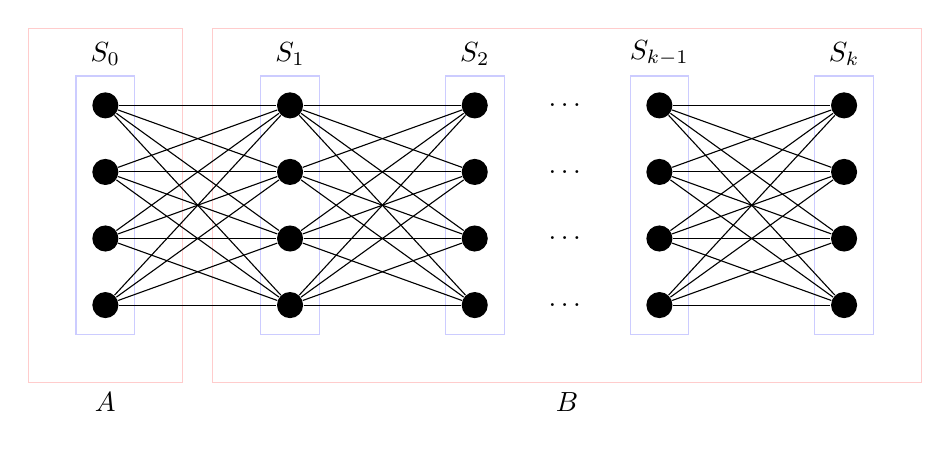
\begin{tikzpicture}[
    roundnode/.style={circle, fill=black, minimum size=0.5mm},
    align=center,
    node distance=0.5cm and 2cm
    ]
    %Nodes
    \node[roundnode] (1A) {};
    \node[roundnode] (1B) [below=of 1A] {};
    \node[roundnode] (1C) [below=of 1B] {};
    \node[roundnode] (1D) [below=of 1C] {};
    
    \node[draw=blue!20,inner sep=2mm,label=above:$S_0$,fit=(1A) (1A) (1A) (1D)] (S0fit) {};

    \node[draw=red!20,inner sep=6mm,label=below:$A$,fit=(S0fit)] {};
    
    \node[roundnode] (2A) [right=of 1A]{};
    \node[roundnode] (2B) [below=of 2A] {};
    \node[roundnode] (2C) [below=of 2B] {};
    \node[roundnode] (2D) [below=of 2C] {};
    
    \node[draw=blue!20,inner sep=2mm,label=above:$S_1$,fit=(2A) (2A) (2A) (2D)] (S1fit) {};
    
    \node[roundnode] (3A) [right=of 2A]{};
    \node[roundnode] (3B) [below=of 3A] {};
    \node[roundnode] (3C) [below=of 3B] {};
    \node[roundnode] (3D) [below=of 3C] {};
    
    \node[draw=blue!20,inner sep=2mm,label=above:$S_2$,fit=(3A) (3A) (3A) (3D)] {};
    
    \node[roundnode] (4A) [right=of 3A]{};
    \node[roundnode] (4B) [below=of 4A] {};
    \node[roundnode] (4C) [below=of 4B] {};
    \node[roundnode] (4D) [below=of 4C] {};
    
    \path (3A) -- node[auto=false]{\ldots} (4A);
    \path (3B) -- node[auto=false]{\ldots} (4B);
    \path (3C) -- node[auto=false]{\ldots} (4C);
    \path (3D) -- node[auto=false]{\ldots} (4D);
    
    \node[draw=blue!20,inner sep=2mm,label=above:$S_{k-1}$,fit=(4A) (4A) (4A) (4D)] {};
    
    \node[roundnode] (5A) [right=of 4A]{};
    \node[roundnode] (5B) [below=of 5A] {};
    \node[roundnode] (5C) [below=of 5B] {};
    \node[roundnode] (5D) [below=of 5C] {};
    
    \node[draw=blue!20,inner sep=2mm,label=above:$S_k$,fit=(5A) (5A) (5A) (5D)] (Skfit) {};
    
    \node[draw=red!20,inner sep=6mm,label=below:$B$,fit=(S1fit) (Skfit)] {};

    %Lines
    \draw[-] (1A) -- (2A);
    \draw[-] (1B) -- (2A);
    \draw[-] (1C) -- (2A);
    \draw[-] (1D) -- (2A);
    \draw[-] (1A) -- (2B);
    \draw[-] (1B) -- (2B);
    \draw[-] (1C) -- (2B);
    \draw[-] (1D) -- (2B);
    \draw[-] (1A) -- (2C);
    \draw[-] (1B) -- (2C);
    \draw[-] (1C) -- (2C);
    \draw[-] (1D) -- (2C);
    \draw[-] (1A) -- (2D);
    \draw[-] (1B) -- (2D);
    \draw[-] (1C) -- (2D);
    \draw[-] (1D) -- (2D);
    
    
    \draw[-] (2A) -- (3A);
    \draw[-] (2B) -- (3A);
    \draw[-] (2C) -- (3A);
    \draw[-] (2D) -- (3A);
    \draw[-] (2A) -- (3B);
    \draw[-] (2B) -- (3B);
    \draw[-] (2C) -- (3B);
    \draw[-] (2D) -- (3B);
    \draw[-] (2A) -- (3C);
    \draw[-] (2B) -- (3C);
    \draw[-] (2C) -- (3C);
    \draw[-] (2D) -- (3C);
    \draw[-] (2A) -- (3D);
    \draw[-] (2B) -- (3D);
    \draw[-] (2C) -- (3D);
    \draw[-] (2D) -- (3D);
    
    \draw[-] (4A) -- (5A);
    \draw[-] (4B) -- (5A);
    \draw[-] (4C) -- (5A);
    \draw[-] (4D) -- (5A);
    \draw[-] (4A) -- (5B);
    \draw[-] (4B) -- (5B);
    \draw[-] (4C) -- (5B);
    \draw[-] (4D) -- (5B);
    \draw[-] (4A) -- (5C);
    \draw[-] (4B) -- (5C);
    \draw[-] (4C) -- (5C);
    \draw[-] (4D) -- (5C);
    \draw[-] (4A) -- (5D);
    \draw[-] (4B) -- (5D);
    \draw[-] (4C) -- (5D);
    \draw[-] (4D) -- (5D);

    \end{tikzpicture}
        \caption{Construction of $H_{k, \Delta}(A,B)$ after Step 1}
        \label{fig:HkAB_1}
    \end{figure}
    
	\textit{Step 2.} Let $G_A$ be an arbitrary m-regular % TODO: Fill in once decided on ending graphs
	graph on $A \setminus S_0$ such that $\Phi(G_A) = \Theta(1)$. %TODO: remove this??

	% TODO: m-regular graph 
	% https://sites.math.rutgers.edu/~sk1233/courses/topics-S13/lec8.pdf
	% Margulis–Gabber–Galil convert to simple graph?

	We now connect each node of $S_0$ to $\Delta$ distinct nodes of $G_A$. First, we arbitrarily enumerate the nodes in $S_0$ and $G_A$ as $v_1, v_2, \dots, v_\Delta$ and $u_1, u_2, \dots, u_{|G_A|}$ respectively. Connect $v_1$ to the first $\Delta$ nodes in the $G_A$, starting with $u_1$. Connect $v_2$ to the next $\Delta$ nodes in $G_A$, starting with $u_{\Delta + 1}$.
	Repeat this process for each $v_i$, as in Figure \ref{fig:HkAB_2}.
	If there are more new connections than nodes in $G_A$, reuse nodes in $G_A$ starting again from $u_1$ and forming new connections in the enumerated order, i.e the $i^\text{th}$ new connection should be made with node $u_m$ where $m = i\mod |G_A|$.

    \begin{figure}[h]
        \centering
        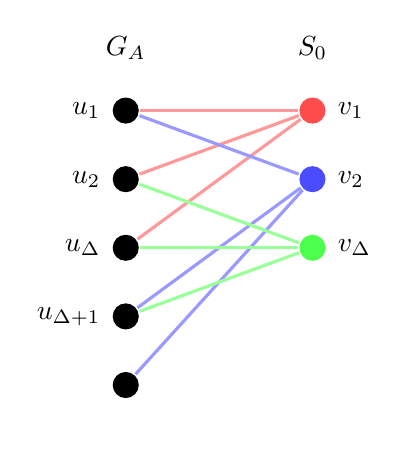
\begin{tikzpicture}[
    roundnode/.style={circle, fill=black, minimum size=0.5mm},
    align=center,
    node distance=0.5cm and 2cm,
    redline/.style={-, red!40},
    blueline/.style={-, blue!40},
    greenline/.style={-, green!40},
    line width = 0.4mm
    ]
    %Nodes
    \node[roundnode, label=west:$u_1$] (1A) {};
    \node[roundnode, label=west:$u_2$] (1B) [below=of 1A] {};
    \node[roundnode, label=west:$u_\Delta$] (1C) [below=of 1B] {};
    \node[roundnode, label=west:$u_{\Delta+1}$] (1D) [below=of 1C] {};
    \node[roundnode] (1E) [below=of 1D] {};

    \node[inner sep=3mm,label=above:$G_A$,fit=(1A) (1A) (1A) (1E)] {};
    
    \node[roundnode, label=east:$v_1$, red!70] (2A) [right=of 1A]{};
    \node[roundnode, label=east:$v_2$, blue!70] (2B) [below=of 2A] {};
    \node[roundnode, label=east:$v_\Delta$, green!70] (2C) [below=of 2B] {};
    
    \node[inner sep=3mm,label=above:$S_0$,fit=(2A) (2A) (2A) (2C)] {};
    
    %Lines
    \draw[redline] (1A) -- (2A);
    \draw[redline] (1B) -- (2A);
    \draw[redline] (1C) -- (2A);

    \draw[blueline] (1D) -- (2B);
    \draw[blueline] (1E) -- (2B);
    \draw[blueline] (1A) -- (2B);

    \draw[greenline] (1B) -- (2C);
    \draw[greenline] (1C) -- (2C);
    \draw[greenline] (1D) -- (2C);

\end{tikzpicture}
        \caption{Illustration of the enumeration technique used in Step 2}
        \label{fig:HkAB_2}
    \end{figure}


	\textit{Step 3.} Let $G_B$ be an arbitrary m-regular graph on $B \setminus \bigcup_{i=1}^k S_i$ such that $\Phi(G_B) = \Theta(1)$. 
	We generate $G_B$ using the same construction as in Step 2. We then connect each node of $S_k$ to $\Delta$ distinct nodes of $G_B$ using the same enumeration method as in Step 2. This yields the graph $H_{k, \Delta}(A,B)$ illustrated in Figure \ref{fig:HkAB_3}.

    \begin{figure}[h]
        \centering
        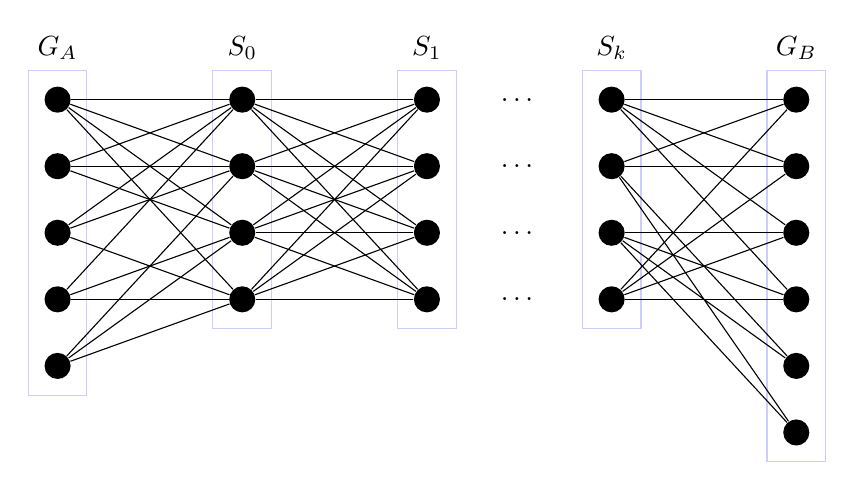
\begin{tikzpicture}[
    roundnode/.style={circle, fill=black, minimum size=0.5mm},
    align=center,
    node distance=0.5cm and 2cm
    ]
    %Nodes
    \node[roundnode] (1A) {};
    \node[roundnode] (1B) [below=of 1A] {};
    \node[roundnode] (1C) [below=of 1B] {};
    \node[roundnode] (1D) [below=of 1C] {};
    \node[roundnode] (1E) [below=of 1D] {};

    \node[draw=blue!20,inner sep=2mm,label=above:$G_A$,fit=(1A) (1A) (1A) (1E)] {};
    
    \node[roundnode] (2A) [right=of 1A]{};
    \node[roundnode] (2B) [below=of 2A] {};
    \node[roundnode] (2C) [below=of 2B] {};
    \node[roundnode] (2D) [below=of 2C] {};
    
    \node[draw=blue!20,inner sep=2mm,label=above:$S_0$,fit=(2A) (2A) (2A) (2D)] {};
    
    \node[roundnode] (3A) [right=of 2A]{};
    \node[roundnode] (3B) [below=of 3A] {};
    \node[roundnode] (3C) [below=of 3B] {};
    \node[roundnode] (3D) [below=of 3C] {};
    
    \node[draw=blue!20,inner sep=2mm,label=above:$S_1$,fit=(3A) (3A) (3A) (3D)] {};
    
    \node[roundnode] (4A) [right=of 3A]{};
    \node[roundnode] (4B) [below=of 4A] {};
    \node[roundnode] (4C) [below=of 4B] {};
    \node[roundnode] (4D) [below=of 4C] {};
    
    \path (3A) -- node[auto=false]{\ldots} (4A);
    \path (3B) -- node[auto=false]{\ldots} (4B);
    \path (3C) -- node[auto=false]{\ldots} (4C);
    \path (3D) -- node[auto=false]{\ldots} (4D);
    
    \node[draw=blue!20,inner sep=2mm,label=above:$S_k$,fit=(4A) (4A) (4A) (4D)] {};
    
    \node[roundnode] (5A) [right=of 4A]{};
    \node[roundnode] (5B) [below=of 5A] {};
    \node[roundnode] (5C) [below=of 5B] {};
    \node[roundnode] (5D) [below=of 5C] {};
    \node[roundnode] (5E) [below=of 5D] {};
    \node[roundnode] (5F) [below=of 5E] {};
    
    \node[draw=blue!20,inner sep=2mm,label=above:$G_B$,fit=(5A) (5A) (5A) (5F)] {};
    
    
    %Lines
    \draw[-] (1A) -- (2A);
    \draw[-] (1B) -- (2A);
    \draw[-] (1C) -- (2A);
    \draw[-] (1D) -- (2A);

    \draw[-] (1A) -- (2B);
    \draw[-] (1B) -- (2B);
    \draw[-] (1C) -- (2B);
    \draw[-] (1E) -- (2B);

    \draw[-] (1A) -- (2C);
    \draw[-] (1B) -- (2C);
    \draw[-] (1D) -- (2C);
    \draw[-] (1E) -- (2C);

    \draw[-] (1A) -- (2D);
    \draw[-] (1C) -- (2D);
    \draw[-] (1D) -- (2D);
    \draw[-] (1E) -- (2D);
    
    \draw[-] (2A) -- (3A);
    \draw[-] (2B) -- (3A);
    \draw[-] (2C) -- (3A);
    \draw[-] (2D) -- (3A);
    \draw[-] (2A) -- (3B);
    \draw[-] (2B) -- (3B);
    \draw[-] (2C) -- (3B);
    \draw[-] (2D) -- (3B);
    \draw[-] (2A) -- (3C);
    \draw[-] (2B) -- (3C);
    \draw[-] (2C) -- (3C);
    \draw[-] (2D) -- (3C);
    \draw[-] (2A) -- (3D);
    \draw[-] (2B) -- (3D);
    \draw[-] (2C) -- (3D);
    \draw[-] (2D) -- (3D);
    
    \draw[-] (4A) -- (5A);
    \draw[-] (4A) -- (5B);
    \draw[-] (4A) -- (5C);
    \draw[-] (4A) -- (5D);

    \draw[-] (4B) -- (5E);
    \draw[-] (4B) -- (5F);
    \draw[-] (4B) -- (5A);
    \draw[-] (4B) -- (5B);

    \draw[-] (4C) -- (5C);
    \draw[-] (4C) -- (5D);
    \draw[-] (4C) -- (5E);
    \draw[-] (4C) -- (5F);

    \draw[-] (4D) -- (5A);
    \draw[-] (4D) -- (5B);
    \draw[-] (4D) -- (5C);
    \draw[-] (4D) -- (5D);

    \end{tikzpicture}
        \caption{Construction of $H_{k, \Delta}(A,B)$ after Step 3}
        \label{fig:HkAB_3}
    \end{figure}

	%TODO: explain how Winding around the ring increases the degree by at most an additive constant O(sqrt(n))^2 extra edges O(n) nodes in A \ S_0 so by O notation at most addivie constant difference

\end{definition}

We note that Definition \ref{def:HkAB} technically specifies a family of graphs, since the construction relies on choosing arbitrary sets of vertices, each of which yields a distinct graph. However, for the purposes of this analysis we think of $H_{k, \Delta}(A,B)$ as a single graph as all graphs in the family have the same structural properties required for the proof, so we can choose any of them. % TODO: Remove this paragraph? premature?

Using $H_{k, \Delta}(A,B)$, we now construct the following dynamic network for which Theorem \ref{theorem:AsyncUpperBound} is tight.

\begin{definition}
	$\rho$-diligent Dynamic Network
	
	First we define the sequences of node subsets $(A_t)_{t\geq 0}$ and $(B_t)_{t\geq0}$ with $A_t, B_t \subseteq V$ for all $t$. For each $t$, we construct $A_t$ and $B_t$ such that they partition $V$ into two subsets, as follows:

	Let $A_0$ be an arbitrary subset of $V$ of size $\floor{\frac{n}{4}}$ containing the first node to be aware of the rumour. % TODO: Any problem with ceiling function?
	Set $B_0 = V \setminus A_0$. Let $B_{t+1} = B_t \setminus I_{t+1}$, i.e. the set of nodes in $B_t$ that were still not informed of the rumour by round $t+1$. % TODO: Have we defined what I_t is?
	Let $A_{t+1} = V \setminus A_t$, i.e. the set of nodes that were either in $A_0$ or informed of the rumour by round $t+1$.

	Now we can define the dynamic network $\rho$-diligent Dynamic Network $\mathcal{G}(n, \rho) = (G_t)_{t\geq 0}$ itself. 
	% TODO: Check sequnce notation consistent, 0 not in N
	% TODO: Does \Delta satisfy conditions required for H_\Delta(A,B)
	% TODO: Standardise notation for H_K(A,B)

	Let $\Delta = \ceil{\frac{1}{\rho}}$, and $k = \mathcal{O}(\log n / \log \log n)$.
	Let $G_t = H_{k, \Delta}(A_t, B_t)$ while $|B_t| \geq \frac{n}{4}$. Note that since $\Delta = \mathcal{O}(\sqrt{n})$ by the definition of $H_{k, \Delta}(A,B)$, we must have that $\rho = \Omega\left(\frac{1}{\sqrt{n}}\right)$.
	Note also that $|A_t|$ is increasing in $t$ since $A_t$ is a superset of the informed nodes at time $t$, so there may be some time step $l$ where $|A_l| > \ceil{\frac{3n}{4}}$. Thus, for all time steps $t \geq l$, we cannot construct $H_{k, \Delta}(A_t,B_t)$. Hence, for all $t \geq l$, let $G_{t+1} = G_t$.
\end{definition}

In the following theorem, we use Theorem \ref{theorem:AsyncUpperBound} to bound the rumour spreading time of Algorithm \ref{NodeCentricAsyncAlgorithm} on a $\rho$-diligent dynamic network.

\begin{theorem}
	w.h.p, the rumour spreading time of Algorithm \ref{NodeCentricAsyncAlgorithm} on a $\rho$-diligent dynamic network with $n$ vertices, where $\rho = \Omega(\frac{1}{\sqrt{n}})$, is at most 
	$$
		\mathcal{O}\left(\left(\rho n + \frac{k}{\rho}\right)\log n\right)
	$$
\end{theorem}

\begin{proof}
	To determine a concrete bound using Theorem \ref{theorem:AsyncUpperBound}, we need to calculate $\Phi(G_t)$ and $\rho(G_t)$. Since $G_t = H_{k, \Delta}(A, B)$ for some $A$ and $B$ at each time step, it suffices to calculate the conductance and diligence for a general $H_{k, \Delta}(A, B)$.

	\textbf{Claim 1.} $\Phi(H_{k, \Delta}(A, B)) = \Theta\left(\frac{\Delta^2}{k\Delta^2 +n }\right)$

	For $q = 1, \dots, k$, let $A_q = G_A \cup \bigcup_{i=1}^q  S_i$. We want to calculate $\text{vol}(A_q)$. The degree of any arbitrary node in $S_i$ is $2\Delta$, since it is connected to all $\Delta$ nodes in $S_{i-1}$ and all $\Delta$ nodes in $S_{i+1}$, where we set $S_0 = G_A$ and $S_{k+1} = G_B$ for brevity. Since there are $\Delta$ nodes in each $S_i$, $\text{vol}(S_i) = 2\Delta^2$. By taking the disjoint union of $q$ $S_i$ subsets, we obtain that $\text{vol}(\bigcup_{i=1}^q) = 2q\Delta^2$. Now we consider $\text{vol}(G_A)$. Since $|A| = \Theta(n)$ and $|S_i| = \Delta = \mathcal{O}(\sqrt{n})$, 
	$$
		|G_A| = |A \setminus S_0| = |A| - |S_0| = \Theta(n) - \mathcal{O}(\sqrt{n}) = \Theta(n)
	$$
	By construction each node in $G_A$ is connected to exactly $m$ % TODO: Replace with actual number
	other nodes in $G_A$, so internal edges contribute $\Theta(n)$ degree to $\text{vol}(G_A)$. The only other edges which terminate in $G_A$ are the $\Delta^2$ edges between $G_A$ and $S_0$, thus $\text{vol}(G_A) = \Delta^2 + \Theta(n)$. By taking the disjoint union of $G_A$ and $\bigcup_{i=1}^q S_i$ we obtain $\text{vol}(A_q) = (2q + 1)\Delta^2 + \Theta(n)$. % TODO: Check as doesn't match paper.
	
	Note that for any $q$, $|E(A_q,\comp{A_q})| = \Delta^2$ since the only edges connecting $A_q$ and $\comp{A_q}$ are the edges passing between $S_q$ and $S_{q+1}$. This is most easily seen by inspecting Figure \ref{fig:HkAB_3}, and noting that $A_q$ corresponds to the first $q + 1$ sets of nodes in the string, while $\comp{A_q}$ corresponds to the remaining $k - q + 1$ sets of noes at the end of the string. By construction, each of these cuts consist of exactly $\Delta^2$ edges, thus $|E(A_q,\comp{A_q})| = \Delta^2$ as claimed.
	Hence, we can derive an upper bound on the conductance of $H_{k, \Delta}(A, B)$ by evaluating the conductance expression for the set $A_q$ instead of the set which achieves the minimum. 
	$$
		\Phi(H_{k, \Delta}(A, B)) \leq \frac{|E(A_q, \comp{A_q})|}{\min \left\{ \text{vol}(A_q), \text{vol}(\comp{A_q}) \right\} } % TODO: THIS INEQUALITY DOESN'T WORK
		\leq \frac{|E(A_q, \comp{A_q})|}{\text{vol}(A_q)} = \frac{\Delta^2}{(2q + 1)\Delta^2 + \Theta(n)}
	$$	
	% TODO: Prove that A_k is the minimal set

	% TODO: Finish this

	\textbf{Claim 2.} $\rho(H_{k, \Delta}(A,B)) = \Theta\left(\frac{1}{\Delta}\right)$

	First we consider the set of vertices $A = G_A \cup S_0$ for which the minimal diligence is achieved. % TODO: Check this works with A instead of A_1 (used in paper)
	We have that $\text{vol}(A) = 2\Delta^2 + \Theta(n)$ since $S_0$ contributes $2\Delta^2$ degree and $G_A$ contributes $\Theta(n)$ degree as shown in claim 1. Since $\Delta = \mathcal{O}(\sqrt{n})$, we obtain that 
	$$
		\text{vol}(A) = 2 \mathcal{O}(\sqrt{n})^2 + \Theta(n) = \mathcal{O}(n) + \Theta(n) = \Theta(n)
	$$ % TODO: Check adding theta and O gives theta
	Since $|A| = \Theta(n)$ by construction we have that the average degree of $A$ satisfies $$
		\bar{d}(A) = \frac{\text{vol}(A)}{|A|} = \frac{\Theta(n)}{\Theta(n)} = \Theta(1)
	$$
	To compute the diligence of $A$, we now consider the cut set $E(A, \comp{A})$. Since every endpoint of the cut set has degree $2\Delta$, we get that 
	$$
		\min_{\{u, v\} \in E(A, \comp{A})} \max \left\{ \frac{1}{d_u}, \frac{1}{d_v} \right\} = \frac{1}{2\Delta}
	$$
	Hence, the diligence of $A$ is 
	$$
		\rho(A) = \frac{\bar{d}(A)}{2\Delta} = \Theta\left(\frac{1}{\Delta}\right)
	$$ 
	
	Now we prove that no set with a smaller diligence exists. First note that we increase the degree of each node in $G_A$ by $\Theta(1)$ when joining them to $S_0$ and $S_1$ in Step 2 of the construction of $H_{k, \Delta}(A,B)$. To see this, we observe that the enumeration technique illustrated in Figure \ref{fig:HkAB_2} spreads the $\Delta^2$ additional edges evenly across $G_A$. Thus, the degree increase for an arbitrary node in $G_A$ is at most
	$$
		\ceil{\frac{\Delta^2}{|G_A|}}=\frac{\mathcal{O}(n)}{\Theta(n)} = \mathcal{O}(1)
	$$
	since $\Delta = \mathcal{O}(\sqrt{n})$ and $|G_A| = \Theta(n)$. 
	
	Since by construction, the internal edges in $G_A$ contribute $\Theta(1)$ degree to each node, we have that the degree for an arbitrary node in $G_A$ is $\Theta(1) + \mathcal{O}(1) = \Theta(1)$. As $G_B$ is connected to the string of bipartite graphs in an identical fashion during Step 2, all nodes of $G_B$ also have $\Theta(1)$ degree.  
	
	Let $S \subseteq V$ be an arbitrary subset of nodes. Since we have that all nodes in $G_A$ and $G_B$ have degree $\Theta(1)$, the maximum degree of any node in the graph is $2\Delta$. Hence 

	$$
	\min_{\{u, v\} \in E(S, \comp{S}) } \left\{ \max \left\{ \frac{1}{d_u},\frac{1}{d_v} \right\} \right\} \geq \frac{1}{2\Delta}
	$$
	Since all nodes have at least constant degree, we have that $\comp{d}(S) = \Omega(1)$. Thus 
	$$
		\rho(S) 
		= \comp{d}(S) \min_{\{u, v\} \in E(S, \comp{S}) } \left\{ \max \left\{ \frac{1}{d_u},\frac{1}{d_v} \right\} \right\}
		\geq \frac{\Omega(1)}{2\Delta}
		= \Omega\left(\frac{1}{\Delta}\right)
	$$
	Thus, since no subset of nodes exists with a lower diligence than the set $A$, our claim holds.

	We can now apply the bound from Theorem \ref{theorem:AsyncUpperBound}, to yield an upper bound on the spreading time of a $\rho$-diligent dynamic network $\mathcal{G}(n, \rho) = (G_t)_{t\geq 0}$. 
	
	From Theorem \ref{theorem:AsyncUpperBound}, we have that the first $T$ for which $\sum_t^T \Phi(G_t)\rho(G_t)$ exceeds $C \log n = \mathcal{O}(\log n)$ is an upper bound on the spreading time w.h.p.  Note that 
	$$
		\sum_t^T \Phi(G_t)\rho(G_t)
		= 
		T \Theta\left(\frac{\Delta^2}{k\Delta^2 +n }\right) \Theta\left(\frac{1}{\Delta}\right)
		= 
		T \Theta\left(\frac{\Delta}{k\Delta^2 +n }\right)
		= 
		T \Theta\left(\frac{1}{n \rho + \frac{k}{\rho}}\right)
	$$
	since $G_t = H_{k, \Delta}(A_t,B_t)$ for all $t$, where $\Delta = \ceil{\frac{1}{\rho}} = \Theta\left(\frac{1}{\rho}\right)$ by the definition of the dynamic network. Hence 
	$$
		\min \left\{T : \sum_t^T \Phi(G_t)\rho(G_t) \geq C \log n \right\}
		=
		\frac{\mathcal{O}(\log n)}{\Theta\left(\frac{1}{n \rho + \frac{k}{\rho}}\right)}
		= 
		\mathcal{O}\left(\log n \left(n \rho + \frac{k}{\rho}\right)\right)
	$$
	% TODO: Resolve k -> 0 log n -> +inf -> (check multaplicitve difference between log n from upper bound and 1/k for lower bound)
	% 		- why choice of log n / log log n for k?
\end{proof}

Now we verify that the upper bound is tight by computing a lower bound on the spreading time for a $\rho$-diligent dynamic network that holds w.h.p.

First we prove a lemma about the spread of the rumour down the chain of bipartite subgraphs in $H_{k, \Delta}(A,B)$.

\begin{lemma}\label{lemma:H_k,DeltaABOneStep}
	Suppose we spread a rumour according to Algorithm \ref{NodeCentricAsyncAlgorithm} on $G = H_{k, \Delta}(A,B)$ for some $A, B$ with $\Delta = \ceil{\frac{1}{\rho}}$. Assume that every node in $S_0$ is aware of the rumour, and no node in $B$ is informed. Then the probability that at least one node of $S_k$ is informed after a unit length of time is at most
	$$
		\frac{2^k}{k!}\ceil{\frac{1}{\rho}}
	$$	
\end{lemma}

\begin{proof}
	% TODO: Introduce two-push algorithm
	Let $I_i(\gamma)$ denote the number of informed nodes in $S_i$ at time $\gamma \in [0,1]$. 
	% Note that, by assumption, we have that $I_0(\gamma) = |S_0| = \Delta$ for all $\gamma \in [0,1]$. 

	We prove the claim by induction on $m$. % TODO: Change "claim" wording to be more specific - talking about expectation

	\underline{Base Case.} $\mathbb{E}I_1(\tau) \leq 2 \tau \Delta$

	Since each node in $S_0$ is aware of the rumour, each of the $\Delta^2$ edges from $S_0$ to $S_1$ is pushing the rumour forward at rate $\frac{2}{\Delta}$ for all times $\gamma \in [0,1]$. Thus, by the superposition property of Poisson processes, the overall rate at which the rumour is pushed from $S_0$ to any node of $S_1$ is $\frac{2}{\Delta}\Delta^2 = 2\Delta$. Let $N_1(\tau)$ denote the number of times any node of $S_1$ is informed of the rumour in the interval $[0,\tau]$ (even if it already knew the rumour). By the theory of Poisson processes, $N_1(\tau)$ is distributed according to a Poisson distribution with mean $2\tau\Delta$. Note $I_i(\tau) \leq N_1(\tau)$ since the same nodes of $S_1$ may be contacted multiple times. Hence $\mathbb{E}I_1(\tau) \leq \mathbb{E}N_1(\tau) = 2\tau\Delta$ as required.
	
	\underline{Inductive Case.} $\mathbb{E}I_k(\tau) \leq \frac{2^k \tau^k}{k!}\Delta$

	Assume that for all $m \leq k - 1$ and $\gamma \in [0,1]$, $\mathbb{E}I_m(\gamma) \leq \frac{2^m \gamma^m}{m!}\Delta$ holds.
	By the tower law,
	$$
		\mathbb{E}I_k(\tau) = \mathbb{E}\mathbb{E}[I_k(\tau) |I_{k-1}(\gamma), \gamma \in [0, \tau]] % TODO: [0, \tau] or [0,1] like in the paper
	$$
	As in the base case, let $N_k(\tau)$ denote the number of times a node in $S_k$ is informed of the rumour in the interval $[0, \tau]$. Since $I_k(\tau) \leq N_k(\tau)$,
	$$
		\mathbb{E}[I_k(\tau) |I_{k-1}(\gamma), \gamma \in [0, 1]] \leq \mathbb{E}[N_k(\tau) |I_{k-1}(\gamma), \gamma \in [0, \tau]]
	$$
	At time $\gamma \in [0,1]$, there are $I_{k-1}(\gamma)$ nodes aware of the rumour in $S_{k-1}$, and pushing the rumour down each of their $\Delta$ edges to $S_k$. Since each of these edges pushes the rumour according to a Poisson process of rate $\frac{2}{\Delta}$, by the superposition of Poisson processes the nodes of $S_{k-1}$ inform the nodes of $S_k$ according to a Poisson processes of rate $\frac{2}{\Delta}I_{k-1}(\gamma)\Delta = 2 I_{k-1}(\gamma)$.
	Thus, $N_k(\tau)|(I_{k-1}(\gamma), \gamma \in [0, \tau])$ is an inhomogeneous Poisson process, where the value of the rate function at time $\gamma$ is $2 I_{k-1}(\gamma)$. By % TODO: CITE HOMOGENEOUS THEOREM
	, 
	\begin{align*}
		\mathbb{E}[N_k(\tau)|I_{k-1}(\gamma), \gamma \in [0, \tau]] &= \mathbb{E}\int_0^\tau 2 I_{k-1}(\gamma) d\gamma \\
		&= 2 \int_0^\tau \mathbb{E}I_{k-1}(\gamma) d\gamma \\ % TODO: How can we swap integral and expectation? Fubinis theorem since I_{k-1}(\gamma) \leq \Delta
		& \leq 2 \int_0^\tau \frac{2^{k-1} \gamma^{k-1}}{(k-1)!} \Delta d\gamma \\
		\intertext{by the induction hypothesis}
		& = \frac{2^k \tau^k}{k!} \Delta
	\end{align*}
	Hence 
	$$
		\mathbb{E}I_k(\tau) \leq \mathbb{E}\frac{2^k \tau^k}{k!}\Delta = \frac{2^k \tau^k}{k!}\Delta
	$$

	% TODO: Prove choice of k and wrap up
\end{proof}


% TODO: Talk about restrictions on rho and k later?
\begin{theorem}
	w.h.p, the rumour spreading time of Algorithm \ref{NodeCentricAsyncAlgorithm} on a $\rho$-diligent dynamic network with $n$ vertices, where $\rho = \Omega(\frac{1}{\sqrt{n}})$, is at least 
	$$
		\Omega\left(\frac{n \rho}{k}\right)
	$$
\end{theorem}

% TODO: Interesting dependence on diligence -> higher diligence = longer to spread?

\begin{proof} 
	Let $T_0$ be the first time that all the nodes of $S_0$ are aware of the rumour. To simplify our analysis, suppose that we are at time $T_0$, hence for all remaining time steps we can assume that every node in $S_0$ is aware of the rumour. % TODO: Check this - we choose S_0 artibitratily, instead consider first time all nodes of A are aware of the rumour? (changes size of B?)

	By the definition of a $\rho$-diligent network, at time $t=0$  we have that all the informed nodes are located in $A_0$, and no node of $B_0$ knows the rumour. Thus, by Lemma \ref{lemma:H_k,DeltaABOneStep}, w.h.p at time $t = 1$, no node of $S_k$ is informed of the rumour. Since the only way the rumour can reach the node set $G_B = B \setminus \bigcup_{i=1}^k S_i$ is through $S_k$ (see Figure \ref{fig:HkAB_3}), we can conclude that w.h.p after the first time step no node of $G_B$ is aware of the rumour. Equivalently we can say that the set of nodes $B_0 \cap I_1 \subseteq \bigcup_i^k S_i$, i.e. all nodes of $B_0$ that are aware of the rumour after one time step are confined to the set of $S_i$s in $G_1$. Hence, 
	\begin{equation}\label{eq:firstStepinfectedNodesOfB}
		|B_0 \cap I_1| \leq \left|\bigcup_{i=1}^k S_i\right| = k\Delta
	\end{equation}
	since each of the $k$ disjoint node sets $S_i$ have size $\Delta$. Since $B_1 = B_0 \setminus I_1$
	$$
		|B_1| = |B_0 \setminus I_1| = |B_0| - |B_0 \cap I_1| \geq \frac{3n}{4} - k\Delta
	$$ % TODO: Corrected typo above
	where the final inequality holds due to inequality (\ref{eq:firstStepinfectedNodesOfB}) and the fact that $|B_0| \geq \frac{3n}{4}$. 
	% TODO: Mention S, G_A, G_B different each timestep - chosen arbitrarily

	We now repeat this analysis for the first $\frac{n}{4k\Delta}$ time steps, by first showing that w.h.p no node in $S_k$ is made aware of the rumour in the first $\frac{n}{4k\Delta}$ time steps. Let $\mathcal{A}_t$ denote the event that in time step $t$ some node in $S_k$ is made aware of the rumour. Note that the event 
	$$\mathcal{A} = \left\{S_k \text{ is informed of the rumour any time step } t \leq \frac{n}{4k\Delta} \right\} = \bigcup_{t=1}^\frac{n}{4k\Delta} \mathcal{A}_t
	$$
	hence by the union bound and Lemma \ref{lemma:H_k,DeltaABOneStep},
	$$
		\mathbb{P}(\mathcal{A}) 
		\leq \sum_{t=1}^\frac{n}{4k\Delta} \mathbb{P}(A_t) 
		\leq \frac{n}{4k\Delta}n^{-c}
		= \frac{n^{1-c}}{4k\Delta} \leq n^{1-c}
	$$
	as $k, \Delta \geq 1$. Since $c > 1$ % TODO: Introduce this restriction earlier
	we have that w.h.p in the first $\frac{n}{4k\Delta}$ time steps the rumour does not reach $S_k$. 

	Thus, for $m \leq \frac{n}{4k\Delta}$ we can repeat the previous analysis inductively as follows % TODO: Rephrase this
	$$
		|B_m| = |B_{m-1} \setminus I_m| \geq \frac{3n}{4} - (m-1)k\Delta - k\Delta = \frac{3n}{4} - mk\Delta
	$$
	Note that for $m = \frac{n}{4k\Delta}$, we get that 
	$$
		|B_m| \geq \frac{3n}{4} - \frac{nk\Delta}{4k\Delta} = \frac{n}{2}
	$$
	Thus, w.h.p after $\frac{n}{4k\Delta}$ time steps, there are still at least $\frac{n}{2}$ nodes who are not aware of the rumour (since no node in $B_i$ is aware of the rumour at the beginning of each time step by construction). Hence, we can conclude the algorithm takes at least 
	$$
		\Omega\left(\frac{n}{4k\Delta}\right) = \Omega\left(\frac{n\rho}{k}\right)
	$$
	time to spread the rumour to all nodes of $\mathcal{G}(n, \rho)$, where $\Delta = \ceil{\frac{1}{\rho}}$.
\end{proof}

\begin{theorem}
	For all large $n$ and $\rho = \Omega\left(\frac{1}{\sqrt{n}}\right)$, there exists a dynamic network on $n$ vertices with diligence $\rho$ for which the bound holds up to a factor of 
	$$
		\mathcal{O}\left(\frac{\log n}{\log \log n}\right)
	$$	
\end{theorem}

% TODO: Significance of over all \rho - can't tighten bound if diligence over \rho

\section{Bounding the synchronous flooding time}
\label{SyncFloodingSection}

In this section we consider a new algorithm for rumour spreading on dynamic network known as flooding, which takes place in discrete rounds instead of continuous time. First we introduce algorithm and prove an upper bound for the spreading time on a dynamic network from \cite{syncPaper}. Then we introduce a new type of dynamic network, where the sequence of topologies is not deterministic, but instead follows a distribution. We generalise our flooding bound to this probabilistic class of dynamic networks, and see an extended example of applying the bound.

\subsection{Model}

First we introduce a new algorithm for rumour spreading in discrete rounds (referred to in \cite{asyncPaper} as synchronous spread).

\begin{definition} \label{SyncFloodingAlgorithm}
	Synchronous Flooding Algorithm

	\noindent
	The synchronous flooding algorithm proceeds in rounds on a dynamic network $\mathcal{G} = (G_t)_{t \in \mathbb{N}}$. Initially a single node is aware of the rumour. In round $i$, every node that is aware of the rumour informs all of its neighbours in $G_i$, regardless of whether they already knew the rumour or not.
\end{definition}

We note that the asynchronous rumour spreading algorithm (Algorithm \ref{NodeCentricAsyncAlgorithm}) was probabilistic since the algorithm depended on sources of randomness such as exponential clocks. In contrast, once the dynamic network and initial node from which the rumour spreads are chosen, Algorithm \ref{SyncFloodingAlgorithm} is entirely deterministic. Since the trajectory of the rumour spread is completely determined by the initial conditions, it is reasonable to ask why we would want bounds on the spreading time if we can simply simulate the rumour, and record how long it takes to inform all the nodes. In some cases however, the graph may be so large that simulation is computationally infeasible. 
In such cases, we may be able to take advantage of bounds in terms of the structural properties of graphs instead. % TODO: Said "cases" at beginning of both sentances
Additionally, in section \ref{subsection:MEDNBound}
we analyse rumour spreading on a non-deterministic dynamic network, where the sequence of graphs is not fixed but instead follows some distribution. 
In this case, deterministic bounds will allow us to bound spreading time over the distribution of graph sequences. %TODO: Said "case" again - change

% TODO: Why study flooding time?
% TODO: mention that Flooding only works for synchronus


\subsection{Bound on spreading time for the Flooding Algorithm}

In this section we prove a bound on the spreading time of the flooding algorithm from \cite{syncPaper}, adding details and expanding steps throughout.

First we introduce the notion of an expander graph, which we need to express the bound.

\begin{definition}
	Boundary set $B(S)$

	\noindent 
	Given a graph $G=(V,E)$, the boundary set $B(S)$ of a vertex subset $S \subseteq V$ is defined as the set of vertices outside $S$ connected to a node of $S$ by an edge, i.e
	$$
		B(S) = \left\{u \in V \setminus S : \{u, v\} \in E \text{ for some } v \in S \right\}
	$$
\end{definition}

% TODO: Figure of boundary sets

\begin{definition}
	$(h, k)$-Expander

	\noindent
	A graph $G$ on a vertex set $V$ is a $(h, k)$-expander if all subsets of the nodes $S \subseteq V$ such that $|S| \leq h$ satisfy $|B(I)| \geq k$.
\end{definition}

Intuitively, an $(h, k)$-Expander should be well-connected since each "small" subset of nodes (i.e. less than $k$ nodes) is connected to at least $k$ other nodes outside the set.  

We are now ready give a bound on the rumour spreading time for the flooding algorithm.

\begin{theorem}\label{theorem:DeterministicFloodingBound}
	\ModelIntro Suppose also that there exists an increasing sequence $1 = h_0 \leq h_1 < \dots < h_s = \frac{n}{2}$ and decreasing sequence $k_1 \geq k_2 \geq \dots \geq k_s$ of positive real numbers, such that for all $t \in \mathbb{N}$, $G_t$ is a $(h_i, k_i)$-expander for every $i \in \{1, \dots , s\}$. Then the spreading time of $\mathcal{G}$ under algorithm \ref{SyncFloodingAlgorithm} is
	$$
		\mathcal{O}\left(\sum_{i=1}^s \frac{\log \frac{h_i}{h_{i-1}}}{\log(1+k_i)}\right)
	$$
\end{theorem}

% TODO: Interpretation of how the bound varies for different (h_i, k_i) sequences, how do these emerge?

We notice that there are strong conditions on the connectivity of the dynamic network that must be met for this bound to hold, namely that every topology is an $(h,k)$-expander for multiple $(h, k)$ pairs. Initially these conditions may seem unreasonably strong, however in Section \ref{subsect:floodingBoundEdgeMarkovian} we will see an interesting example where these properties emerge with high probability in a random graph.

\begin{proof}
	For $i = 1,\dots, s$, let $T_i$ be the earliest time step such that the number of informed nodes is larger than $h_i$, i.e

	$$
		T_i = \min \{ t \in \mathbb{N} : |I_t| > h_i \}
	$$

	First we upper-bound the number of steps in the interval $[T_i, T_j]$, % TODO: Generalise to [T_i, T_j], should all hold as expected
	by bounding the number of informed nodes $t$ time-steps after $T_i$ from below.

	By induction, we show that if $T_i + t < T_j$, then the number of informed nodes at time $T_i + t$ is greater than $(1+k_j)^t h_i$.
	
	\underline{Base Case.} Suppose that $t=0$. 
	
	Then by the definition of $T_i$, the number of informed nodes at time $T_i$ is strictly greater than $h_i$

	\underline{Inductive Case.} For brevity, let $s = T_i + t$. Suppose that $|I_s| > (1+k_j)^t h_i$.

	We notice that 
	% TODO: Justify steps
	\begin{align*}
		|I_{s+1}| &= |I_s| + |B(I_s)| \\ %by operation of algo
		& \geq |I_s| + k_j |I_s| \\ % since we assume s < T_j => |I_s| \leq h_j + (h_j, k_j)-expander
		& = (1 + k_j)|I_s| \\
		& > (1 + k_j)(1+k_j)^t h_i \\ % by induction hypotheis
		& = (1+k_j)^{t+1} h_i
	\end{align*}
	% TODO: boundary set picture here	
	Let $\tau = T_i + \ceil{ \frac{\log (h_j/h_i)}{\log(1+k_j)}}$. 
	Suppose for contradiction that $\tau < T_j$. %TODO: Is contradicition overkill here?
	Since we assumed $\tau < T_j$ we can apply the above inequality %TODO: label
	to get the following lower bound on the number of informed nodes at time $\tau$.
	$$
		|I_\tau| > 
		(1+k_j)^{\ceil{ \frac{\log (h_j/h_i)}{\log(1+k_j)}}} h_i
		\geq e^{\log (h_j/h_i)} h_i
		= h_j
	$$
	Thus we have a contradiction, since under the assumption that $\tau < T_j$, we get that the number of informed nodes at time $\tau$ is greater than $h_j$, i.e. by the definition of $T_j$, $\tau \geq T_j$. Hence, we have that $\tau \geq T_j$ i.e. $\ceil{ \frac{\log (h_j/h_i)}{\log(1+k_j)}}$ time-steps after $T_i$, the number of informed nodes is greater than $h_j$. Rearranging this inequality gives us the following bound on the length of the interval $[T_i, T_j]$:
	\begin{equation} \label{eq:FloodingIntervalBound}
		T_j - T_i \leq \ceil{ \frac{\log (h_j/h_i)}{\log(1+k_j)}} \leq \frac{\log (h_j/h_i)}{\log(1+k_j)} + 1
	\end{equation}
	% TODO: Make ceiling brackets fit
	% TODO: Exposition about next steps + direction here

	% TODO: What about time until first spread - must happen at timestep 2 since (h,k) expander so no isolated nodes.
	Note that since $h_s = \frac{n}{2}$, at time $T_s$ at least half of the nodes will be aware of the rumour. Hence, if we can bound $[T_0, T_s]$, we will have bounded the time it takes for half of the nodes to be informed. 

	To bound $[T_0, T_s]$, we bound each subinterval $[T_{i-1}, T_i]$. Naively applying the bound to each subinterval directly and taking the sum yields the overall bound 
	$$
		\mathcal{O}\left(\sum_{i=1}^s \frac{\log \frac{h_i}{h_{i-1}}}{\log(1+k_i)} + s\right)
	$$ 
	for the interval $[T_0,T_s]$. However, we can tighten the bound by removing the additive $s$ term through case analysis on the subinterval $[T_{i-1}, T_i]$, as follows.

	% TODO: Link back to theorem, after since n/2 = h_s, after T_s at least n/2 nodes are informed


	% TODO: Note that the source of the problems is the cieling function - aim to get into form like in thm statement, but can't naively add all togethe oterwise + O(S) error, requires deeper analysis

	\textbf{Case 1.} Suppose $\frac{\log (h_i/h_{i-1})}{\log(1+k_i)} \geq 1$.

	In this case $\frac{\log (h_i/h_{i-1})}{\log(1+k_i)}$ term is the dominant term in inequality (\ref{eq:FloodingIntervalBound}), thus
	$$
		T_i - T_{i-1} = \mathcal{O}\left( \frac{\log (h_i/h_{i-1})}{\log(1+k_i) }\right) + \mathcal{O}(1) = \mathcal{O}\left( \frac{\log (h_i/h_{i-1})}{\log(1+k_i) }\right)
	$$

	\textbf{Case 2.} Suppose $\frac{\log (h_i/h_{i-1})}{\log(1+k_i)} < 1$.

	In this case we cannot achieve the same bound on $T_i - T_{i-1}$, since the additive 1 is the dominant term. By following the same reasoning as in Case 1, instead we can only obtain that
	\begin{equation}\label{eq:Weak1StepBound}
		T_i - T_{i-1} = \mathcal{O}\left( \frac{\log (h_i/h_{i-1})}{\log(1+k_i) }\right) + \mathcal{O}(1) = \mathcal{O}(1)
	\end{equation}
	To understand the situation that this case represents, we inspect the inequality we assumed.
	By rearranging we find that $(1+k_i)h_{i-1} > h_i$. Since we have assumed that $T_{i-1} < T_i$, % TODO: Assume this earlier
	the number of informed nodes at the start of round $T_{i-1}$ satisfies
	$$
		|I_{T_{i-1}}| \leq h_i
	$$
	Hence, as the topology is an in $(h_i, k_i)$-expander, in round $T_{i-1}$ at least $|I_{T_{i-1}}|k_i$ new uninformed nodes on the boundary of the informed node set are informed. Thus, at the start of the next round, there are at least $(1+k_i)h_{i-1}$ informed nodes, since $|I_{T_{i-1}}| > h_{i-1}$ by the definition of $T_{i-1}$. Combining this with the rearranged form of the assumed inequality, we see that the number of informed nodes "jumps" to more than $h_i$ nodes in a single time step.

	It may be that after this jump there are also more than $h_j$ nodes for some $j \geq i$, %TODO: insert figure here of t vs |I_t|, for t = T_{i-1}, T_i, T_{i+1}, etc, maybe similar figure for steps in case 1.
	from which we obtain $T_{i-1} + 1 = T_i = T_{i+1} = \dots = T_j$. See Figure \ref{fig:floodingJump} for an illustration of this "jump" behaviour. 
	\begin{figure}[h]
		\centering
		\includegraphics[width=1\textwidth]{./figures/flooding_jump.png}
		\caption{Behaviour of the number of informed nodes in the "jump" case}
		\label{fig:floodingJump}
	\end{figure}
	In this case the total time that has passed between $T_{i-1}$ and $T_j$ is 1, so we instead bound the whole jump interval as follows:
	
	% TODO: j doesn't exist case
	Let $j$ be the index such that $h_j < (1+k_i)h_{i-1} \leq h_{j+1}$, i.e. the last $j \geq i$ when $T_j = T_{i-1} + 1$, as in Figure \ref{fig:floodingJump}. % TODO: Check this equivalence - think it does hold
	% TODO: Figure here to illusttrate T_j, 
	% TODO: "may be the same as before" - what does this mean??? 
	Hence, by the definition of $j$, h
	\begin{align*}
		T_j - T_{i-1} &=1 \\ 
		&\leq \frac{\log (h_{j+1}) - \log(h_{i-1})}{\log(1+k_i) } \\
		& =\sum_{l=i}^{j+1} \frac{\log (h_{l}) - \log(h_{l-1})}{\log(1+k_i) } & \text{since the numerator forms a telescoping sum} \\
		& \leq \sum_{l=i}^{j+1} \frac{\log (h_{l}/h_{l-1})}{\log(1+k_l) } & \text{since } k_i \geq k_l \text{ for all } l \geq i \\
		& = \mathcal{O}\left(\sum_{l=i}^j \frac{\log (h_{l}/h_{l-1})}{\log(1+k_l) }\right)
 	\end{align*}

	We now use this equality to bound the growth of $T_s$, the first time at which more than $h_s = \frac{n}{2}$ nodes are aware of the rumour. We can express $T_s$ as a telescoping sum of intervals as follows:
	$$
		T_s = \sum_{i=1}^s T_i - T_{i-1}
	$$
	For the $i^\text{th}$ interval, if $\frac{\log (h_i/h_{i-1})}{\log(1+k_i)} \geq 1$, we can apply the result from Case 1. If $\frac{\log (h_i/h_{i-1})}{\log(1+k_i)} < 1$, we apply Case 2 to bound the whole jump interval $[T_{i-1}, T_j]$, and continue the summation from $T_j$. % TODO: CHeck, problems from j+1 on case 2 result?

	TODO: FINISH PROOF
	
\end{proof}

\subsection{Review of Markov Chains}

\begin{enumerate}
	\item Definition
	\item Stationary distribution definition and Interpretation
\end{enumerate}

\subsection{Flooding on Markovian Evolving Dynamic Networks}

Until now, all the dynamic networks we have studied have been deterministic, in the sense that the evolution of topologies has been fixed. However, knowing the future topologies of the network may be unrealistic in practice. For example, when considering rumour spread on a real-world network such as the internet, we cannot say with certainty what connections will be present on a given time in the future. This motivates a generalistion of the dynamic network model where the sequence of topologies is drawn from some distribution. This distribution expresses our uncertainty in the future topologies of the network, but allows us to encode information about how we predict the shape of the network may evolve. Under this model, the dynamic network itself is a stochastic process, and a source of randomness. In this section, we analyse the rumour spreading time when a Markov chain is used to  generate the random sequence of topologies.

First we introduce a variation of the original Dynamic Network definition.

\label{subsection:MEDNBound}

\begin{definition}
	Markovian Evolving Dynamic Network (MEDN)

	\noindent 
	Let $\mathcal{A}(V)$ be the set of all possible graphs on the vertex set $V$.
	A Markovian Evolving Dynamic Network is a random sequence of graphs $\mathcal{M} = (G_t)_{t \in \mathbb{N}}$ indexed by an integer time $t$, such that $\mathcal{G}$ is a Markov chain with state space $\mathcal{A}(V)$.
\end{definition}

We see that this definition adheres to the previous restriction that all topologies have the same vertex set. Since the network is Markovian, the distribution from which the next topology is draw depends only on the previous topology.

We say that a given MEDN $\mathcal{M}$ is stationary if the distribution of $G_0$ is a stationary distribution of $\mathcal{M}$. By the definition of a stationary distribution, in such an MEDN the probability that $G_t = G'$ for a given $G'$ is the probability that $G_t = G'$ under the stationary distribution, for any time step $t$. Hence, once the Markov chain associated with the network has reached equilibrium, % TODO: define "equalibrium"
the future evolution of the network effectively proceeds by independently sampling a topology from the stationary distribution at each time step. % TODO: Check if independent, get rid of "effectively"?

Under certain conditions, Markov chains converge to their stationary distributions. Thus, for the rest of this section we assume that our MEDNs have been running for a long enough such that when we inject the rumour the network is already in equilibrium. In this paper we don't discuss the conditions which allow for converge to the stationary distribution or how long the convergence takes, and assume that round 0 begins when we inject the rumour.
% TODO: What about if we started not in the stationary distributuion?? Further exploration needed. Or close to stationary? 

We now adapt the deterministic bound proved Theorem \ref{theorem:DeterministicFloodingBound} to a MEDN, by adding details to proof from \cite{syncPaper}

% TODO: Is this a non-theorm? What does it acutally mean?

\begin{theorem}\label{theorem:markovSyncBound}
	Let $\mathcal{M} = (G_t)_{t \in \mathbb{N}}$  be a stationary Markovian evolving graph. Suppose also that there exists an increasing sequence $1 = h_0 \leq h_1 < \dots < h_s = \frac{n}{2}$ and decreasing sequence $k_1 \geq k_2 \geq \dots \geq k_s$ of positive real numbers, such that with probability $1-\frac{1}{n^2}$, the stationary distribution of $\mathcal{M}$ is a $(h_i, k_i)$-expander for every $i \in \{1, \dots , s\}$. Then the spreading time of $\mathcal{G}$ under algorithm \ref{SyncFloodingAlgorithm} is
	$$
		\mathcal{O}\left(\sum_{i=1}^s \frac{\log \frac{h_i}{h_{i-1}}}{\log(1+k_i)}\right)
	$$
	with high probability.
\end{theorem}

Note that in previous bounds the source of randomness in the spreading time has been the rumour spreading algorithm, however in this bound the only source of randomness is the network itself.

We notice that in this theorem, instead of requiring every graph topology to satisfy the expansion conditions of Theorem \ref{theorem:DeterministicFloodingBound}, we only require that the same expansion properties hold with high probability with respect to the stationary distribution. % TODO: REWORD??
Since each topology is sampled from the stationary distribution, these properties will hold for nearly all the topologies in the sequence. Thus, this theorem states that our deterministic bound will hold for MEDNs, as long as the long-term proportion of topologies in our network without strong expansion properties is bounded by $\frac{1}{n^2}$.

% TODO: Review this proof for order that makes sense, and check it actually holds

\begin{proof}
	For all $t \in \mathbb{N}$, let $A_t$ be the event that $G_t$ is an $(h_i, k_i)$-expander for all $1 \leq i \leq s$. Since $\mathcal{M}$ is stationary, we have that $\mathbb{P}(A_t) \geq 1 - \frac{1}{n^2}$ for all t. 

	Let $B$ denote the event we are interested in, namely that the rumour spreading time is 	
	$$
		\mathcal{O}\left(\sum_{i=1}^s \frac{\log \frac{h_i}{h_{i-1}}}{\log(1+k_i)}\right)
	$$

	Suppose that $A_k$ holds for all $k \leq n$. We claim that the rumour spreads in at most $n$ time steps with certainty. Since we have assumed that all topologies up to time $n$ are $(h_1, k_1)$-expanders, there are no isolated nodes, as such an isolated node $v$ would form a subset of size $1 \leq h_1$ with $B({v}) = 0 < k_1$, a contradiction. Thus, the network is connected for the first $n$ time steps. Hence, for any time step $t \leq n$ before all nodes are informed of the rumour, $B(I_t) \geq 1$, since there is only 1 connected component so $I_t$ must be connected  to $U_t$ by at least 1 edge. It follows that in each time step at least 1 new node becomes informed of the rumour by the operation of algorithm \ref{SyncFloodingAlgorithm}. Hence, at most $n$ steps are needed to spread the rumour when $A_k$ holds for all $k \leq n$. 

	Let $T$ denote the first time step at which all nodes are informed of the rumour. By Theorem \ref{theorem:DeterministicFloodingBound} we have that if $A_k$ holds for all $k \leq T$, then $T=\mathcal{O}\left(\sum_{i=1}^s \frac{\log (h_i/h_{i-1})}{\log(1+k_i)}\right)$, as once all the nodes have been informed, the expansion properties of the remaining topologies are irrelevant.

	Now we combine the previous two claims. By the first claim if $A_k$ holds for all $k \leq n$ we have that $T \leq n$, thus $A_k$ holds for all $k \leq T$. In this case, by the second claim we obtain that  $T=\mathcal{O}\left(\sum_{i=1}^s \frac{\log (h_i/h_{i-1})}{\log(1+k_i)}\right)$.

	Since we have shown that the event $\bigcap_{t=0}^n A_t \implies B$, we have that $\comp{B} \implies \comp{ \bigcap_{t=0}^n A_t} = \bigcup_{t=0}^n \comp{A_t}$. To finish the proof, we show that the event $\comp{B}$ happens with vanishing probability, thus $B$ happens with high probability.

	\begin{align*}
		\mathbb{P}(\comp{B}) &\leq \mathbb{P}(\bigcup_{t=0}^n \comp{A_t}) & \text{by the inferred implication} \\ 
		& \leq n \mathbb{P}(\comp{A_t}) & \text{by the union bound}\\ 
		& \leq n \frac{1}{n^2} = \frac{1}{n} & \text{by the conditions on the stationary distribution}
	\end{align*}

	% TODO: THINK ABOUT h_0

\end{proof}

\subsection{Applying the bound to the Edge Markovian MEDN}\label{subsect:floodingBoundEdgeMarkovian}

In this section, we apply the bound proved in Theorem \ref{theorem:markovSyncBound} to a specific MEDN called the Edge-Markovian Network. We will also evaluate the quality of the bound by proving a lower bound on the spreading time, and comparing the results with simulations. 

First, we introduce and motivate the model.
\begin{definition}
	Edge-Markovian Network $\mathcal{M}(n, p, q)$

	\noindent
	Let $V$ be a vertex set, and $E = \left\{e : e \subseteq V, |e| = 2 \right\}$ be the set of all possible edges between vertices in $V$. 
	Let $\left\{\{X_e(t)\}_{t \in \mathbb{N}} : e \in E \right\}$ be a set of independent Markov chains on the state space $\{0,1\}$, each with the transition matrix
	\begin{center}
		\begin{tabular}{ c | c c }
		   & 0     & 1 \\ 
		\hline
		 0 & $1 - p$ & $p$ \\  
		 1 & $q$     & $1 - q$  
		\end{tabular}
	\end{center}
	An Edge-Markovian Evolving Network $\mathcal{M}(n, p, q) = \left\{(V, E_t) : t \in \mathbb{N} \right\}$ is a random sequence of graphs on the vertex set $V$ where $E_t = \left\{ e \in E : X_e(t) = 1 \right\}$, i.e. each edge $e$ is only present in the time steps when its associated Markov chain $X_e$ is in state 1.
\end{definition}
The Edge-Markovian Network models the situation when connections between nodes independently fail or are restored. The "birth" and "death" of each edge $e$ is dictated by its associated Markov chain $X_e$, where in each round, a present edge has probability $q$ of failing, and a missing edge has probability $p$ of restoration. Hence, for any given edge, after a geometrically distributed time with parameter $q$, a failure occurs. Restoring the edge takes a geometrically distributed time with parameter $p$ % TODO: WHAT DO FAILING AND RESTORATION MEAN

Since the future state of each edge is only dependent on current state, this Network is appropriate for modelling memoryless Networks where we can assume each edge acts independently with identical dynamics to other edges. For example, in a computer network we could imagine each  connection is randomly disrupted by an issue with probability $q$, and the affected connection is fixed with probability $p$ in each of the subsequent time steps. 

Now we will see that the set of Markov chains associated with the edges induces a Markov chain over the set of possible graphs on $V$, thus the Edge-Markovian Network is an MEDN.

% TODO: REPAIR-DELAY NETWORKS - any edge could fail, takes a few steps to fix, how to model, what is the stationary distribution?

\begin{lemma}
	The Edge-Markovian Network is a MEDN
\end{lemma}

\begin{proof}
	Since all the edges are memoryless, the distribution of which edges will be present in the subsequent round is only dependent on which edges are present currently. %TODO: Reword this
	Thus, the distribution over possible topologies in the following round is only dependent on the topology in the current round.
	Hence, the sequence of topologies is a Markov chain, so the network is an MEDN.
	% TODO: Include transition probabilities
\end{proof}

% TODO: Proof that it is a MEG 

% TODO: Proof of stationary distribution - plug into

Since the Edge-Markovian Network is an MEDN, we can apply Theorem \ref{theorem:markovSyncBound} to bound the spreading time of Algorithm \ref{SyncFloodingAlgorithm}. Before applying the bound, we need to establish the stationary distribution of this network.

\begin{lemma}
	The stationary distribution of $\mathcal{M}(n, p, q)$
\end{lemma}

\begin{proof}
	Let 
	$$
		\pi = \left(\frac{q}{p+q}, \frac{p}{p+q}\right)
	$$ 
	be a distribution over the starting states of $X_e$ for any $t \in \mathbb{N}, e \in E$, % TODO: E not defined here
	where the first component is the probability of starting in state 0, and the second component is the probability of starting in state 1. First we show that $\pi$ is the stationary distribution for all the edge Markov chains.

	Let $M$ be the transition matrix for any of the edge Markov chains. We calculate the distribution over $\{0,1\}$ after a single round starting in distribution $\pi$. Observe that
	$$
		\pi M =
		\begin{bmatrix}
			\frac{q}{p+q} & \frac{p}{p+q}
		\end{bmatrix}
		\begin{bmatrix}
			1 - p & p \\
			q & 1 - q 
		\end{bmatrix}
		= \begin{bmatrix}
			\frac{q}{p+q} & \frac{p}{p+q}
		\end{bmatrix}
		= \pi
	$$
	thus $\pi$ is the stationary distribution of any $X_e$.
	Now we formulate the stationary distribution of the topology Markov chain. When all edges start in the stationary distribution, at any time step $t$, $X_e(t) = 1$ with probability $\frac{p}{p+q}$ by the stationarity of $\pi$. Hence, under this initial distribution, each edge is present with probability $\frac{p}{p+q}$ in any time step. Note that this distribution over the possible topologies is not dependent on the topology of the network at any other time, hence it is stationary.
\end{proof}
% TODO: Prove that stationary distribution of edge-markovian evolution is ER G(n, p/(p+q))
% DEFINE DISTRIBUTUI

\begin{theorem}
	Let $\mathcal{M}(n, p, q)$ be an Edge-Markovian Dynamic Network in its stationary distribution. If $\hat{p} = \frac{p}{p+q} \geq c \frac{\log n}{n}$ for a sufficiently large $c$ then with high probability, the flooding time in $\mathcal{M}(n, p, q)$ is 

	$$
		\mathcal{O}\left(\frac{\log n}{\log n\hat{p}} + \log \log n\hat{p} \right)
	$$
\end{theorem}

TODO: Proof

\begin{proof}
	
\end{proof}

\begin{lemma}
	Let $\hat{p} \geq c\frac{\log n}{n}$ for a sufficiently large $c$.
\end{lemma}

% TODO: What happens if p < c logn/n?
% lower bound on mixing time
% TODO: Why can't generalise to varying t? (Non-homogenous MC)

\subsection{Simulations}

\begin{figure}[h]
	\centering
	\includegraphics[width=1\textwidth]{./figures/flooding_gnp_simulation_results.png}
	\caption{Results of Edge-Markovian Dynamic Network spreading time simulations}
	\label{fig:floodingGnpSimResults}
\end{figure}

TODO: Evaluate tightness of bound for Edge-Markovian evolution

\chapter{Conclusion}\label{chapter:conclusion}

In this section, we summarise the report, highlight the central results, and present ideas for further study.

We started by introducing an asynchronous rumour spreading model for static networks in Chapter \ref{chapter:staticIntro}, and presented a well-known bound on the spreading time. 

Then, in Chapter \ref{chapter:AsyncUpperBound}, we introduced dynamic networks, and presented a randomised algorithm for rumour spreading on such networks. In Theorem \ref{theorem:AsyncUpperBound}, we proved that the rumour spreading time can be bounded w.h.p. using connectivity metrics of the network's topologies, namely the conductance and diligence. We saw that this bound has no use for networks consisting solely of disconnected topologies. An interesting question for further study is whether it is possible to construct spreading time bounds for networks consisting of disconnected topologies. By applying the bound to various networks and comparing it with simulated spreading times, we saw that the tightness of the bound varies depending on the network. For the networks under investigation, we found that the bound was almost tight in adversarial cases, but much weaker in isomorphic non-adversarial networks. 

In Chapter \ref{chapter:asyncBoundTight}, we strengthened the conclusions of Chapter \ref{chapter:AsyncUpperBound} by constructing a family of adversarial networks for which the bound is provably almost tight (Corollary \ref{corollary:edgeMarkovianThetaBound}). We saw that these networks take advantage of dynamic capabilities to slow the spread of the rumour.

In Chapter \ref{chapter:SyncFlooding} we considered an alternative, deterministic model for rumour spreading known as flooding. In Theorem \ref{theorem:DeterministicFloodingBound}, we presented a bound on the spreading time which also depends on the connectivity metrics of the network. 
However, this bound requires strong connectivity properties to hold for every topology in the network.

We then introduced Markovian-Evolving Dynamic Networks (MEDNs), and generalised the flooding bound to this class of randomised networks in Theorem \ref{theorem:markovSyncBound}. We applied the generalised bound to a specific MEDN known as the Edge-Markovian network, with the restriction that $\hat{p} \geq \frac{c\log n}{n}$ for a sufficiently large $c$. Constructing upper bounds on the spreading time for the Edge-Markovian network $\hat{p} \leq \frac{c \log n}{n}$ remains an interesting area for further study. In Corollary \ref{corollary:edgeMarkovianThetaBound}, we showed that the bound was tight by proving a lower bound on the spreading time that holds w.h.p. We concluded the chapter by investigating how the bound behaved for Edge-Markovian networks with different parameters. Here we saw that for the largest value of $\hat{p}$ where the bound is provably tight, the bound did not match the average spreading times as well as it did for simulations with smaller values of $\hat{p}$. Why this is the case forms another interesting question for further study.

% TODO: SWEEP for future study in readthrough

\printbibliography

\end{document}